% This is a LaTeX thesis template for Monash University.
% to be used with Rmarkdown
% This template was produced by Rob Hyndman
% Version: 6 September 2016

\documentclass{monashthesis}

%%%%%%%%%%%%%%%%%%%%%%%%%%%%%%%%%%%%%%%%%%%%%%%%%%%%%%%%%%%%%%%
% Add any LaTeX packages and other preamble here if required
%%%%%%%%%%%%%%%%%%%%%%%%%%%%%%%%%%%%%%%%%%%%%%%%%%%%%%%%%%%%%%%

\author{Weihao Li}
\title{Advances in Artificial Intelligence for Data Visualization: Developing Computer Vision Models to Automate Reading of Data Plots, with Application to Predictive Model Diagnostics}
\degrees{B.Comm. (Hons), Monash University}
\def\degreetitle{PhD}
% Add subject and keywords below
\hypersetup{
     %pdfsubject={The Subject},
     %pdfkeywords={Some Keywords},
     pdfauthor={Weihao Li},
     pdftitle={Advances in Artificial Intelligence for Data Visualization: Developing Computer Vision Models to Automate Reading of Data Plots, with Application to Predictive Model Diagnostics},
     pdfproducer={Bookdown with LaTeX}
}


\bibliography{thesisrefs}

\usepackage{amsthm}
\newtheorem{theorem}{Theorem}[chapter]
\newtheorem{lemma}{Lemma}[chapter]
\newtheorem{corollary}{Corollary}[chapter]
\newtheorem{proposition}{Proposition}[chapter]
\newtheorem{conjecture}{Conjecture}[chapter]
\theoremstyle{definition}
\newtheorem{definition}{Definition}[chapter]
\theoremstyle{definition}
\newtheorem{example}{Example}[chapter]
\theoremstyle{definition}
\newtheorem{exercise}{Exercise}[chapter]
\theoremstyle{definition}
\newtheorem{hypothesis}{Hypothesis}[chapter]
\theoremstyle{remark}
\newtheorem*{remark}{Remark}
\newtheorem*{solution}{Solution}
\begin{document}

\pagenumbering{roman}

\titlepage

{\setstretch{1.2}\sf\tighttoc\doublespacing}

\clearpage\pagenumbering{arabic}\setcounter{page}{0}

\hypertarget{background-and-motivation}{%
\chapter{Background and Motivation}\label{background-and-motivation}}

The introduction of the report is organised as follows. Section \ref{se:predictive-modelling} discusses the predictive modelling culture and the use of data plots in predictive model diagnostics. Section \ref{se:vi} outlines the definition and terminology of visual inference. Section \ref{se:prespecification} presents the justification of the validity of visual inference. Section \ref{se:sampling-from-null} describes the sampling techniques in visual inference with an example of the classical normal linear regression model. Section \ref{se:lineup} introduces the lineup protocol and the estimation of \(p\)-value and power of a visual test. And lastly, Section \ref{se:limitation} points out the limitation of lineup protocol, which is also the motivation of this research, and the need of building an automatic visual inference system.

\hypertarget{se:predictive-modelling}{%
\section{Predictive Modelling and Visual Diagnostics}\label{se:predictive-modelling}}

\textcite{donoho_50_2017} in its summary of data science stated that the concept of the predictive modelling culture could be traced back to an article written by Breiman (2001). In contrast to the generative modelling culture, which aims to develop stochastic models to make inferences about the data generating process, predictive modelling emphasizes the ability of the model to make accurate predictions.

Predictive models are primarily evaluated by predictive accuracy with the use of validation and test data, but in predictive model diagnostics, especially model testing and tuning, data plots play an irreplaceable role. In these diagnostics, though numeric summaries are mostly available and some are even endorsed by finite or asymptotic properties, graphical representation of data is still preferred, or at least needed by researchers, due to its intuitiveness and the possibility for unexpected discoveries which may be abstract and unquantifiable.

However, unlike confirmatory data analysis built upon rigorous statistical procedures, e.g., hypothesis testing, visual diagnostics relies on graphical perception - human's ability to interpret and decode the information embedded in the graph \autocite{cleveland_graphical_1984}, which is to some extent subjective. Further, visual discovery suffers from its unsecured and unconfirmed nature where the degree of the presence of the visual features typically can not be measured quantitatively and objectively, which may lead to over or under-interpretations of the data. One such example is finding an over-interpretation of the separation between gene groups in a two-dimensional projection from a linear discriminant analysis when in fact there are no differences in the expression levels between the gene groups and separation is not an uncommon occurence \autocite{roy_chowdhury_using_2015}.

\hypertarget{se:vi}{%
\section{Visual Inference}\label{se:vi}}

Visual inference was first introduced in a 1999 Joint Statistical Meetings (JSM) talk with the title ``Inference for Data Visualizatino'' by \textcite{buja_inference_1999} as an idea to address the issue of valid inference for visual discoveries of data plots \autocite{gelman_exploratory_2004}. Later, in the Bayesian context, data plots was systematically considered as model diagnostics by taking advantage of the data simulated from the assumed statistical models \autocite{gelman_bayesian_2003,gelman_exploratory_2004}.

It was surprising that the essential components of visual inference had actually been established in \textcite{buja_inference_1999}, but it was not until 10 years later that \textcite{buja_statistical_2009} formalized it as an inferential framework to extend confirmatory statistics to visual discoveries. This framework redefines the test statistics, tests, null distribution, significance levels and \(p\)-value for visual discovery modelled on the confirmatory statistical testing. Figure \ref{fig:parallelism} outlines the parallelism between conventional tests and visual discovery.

\begin{figure}
\centering
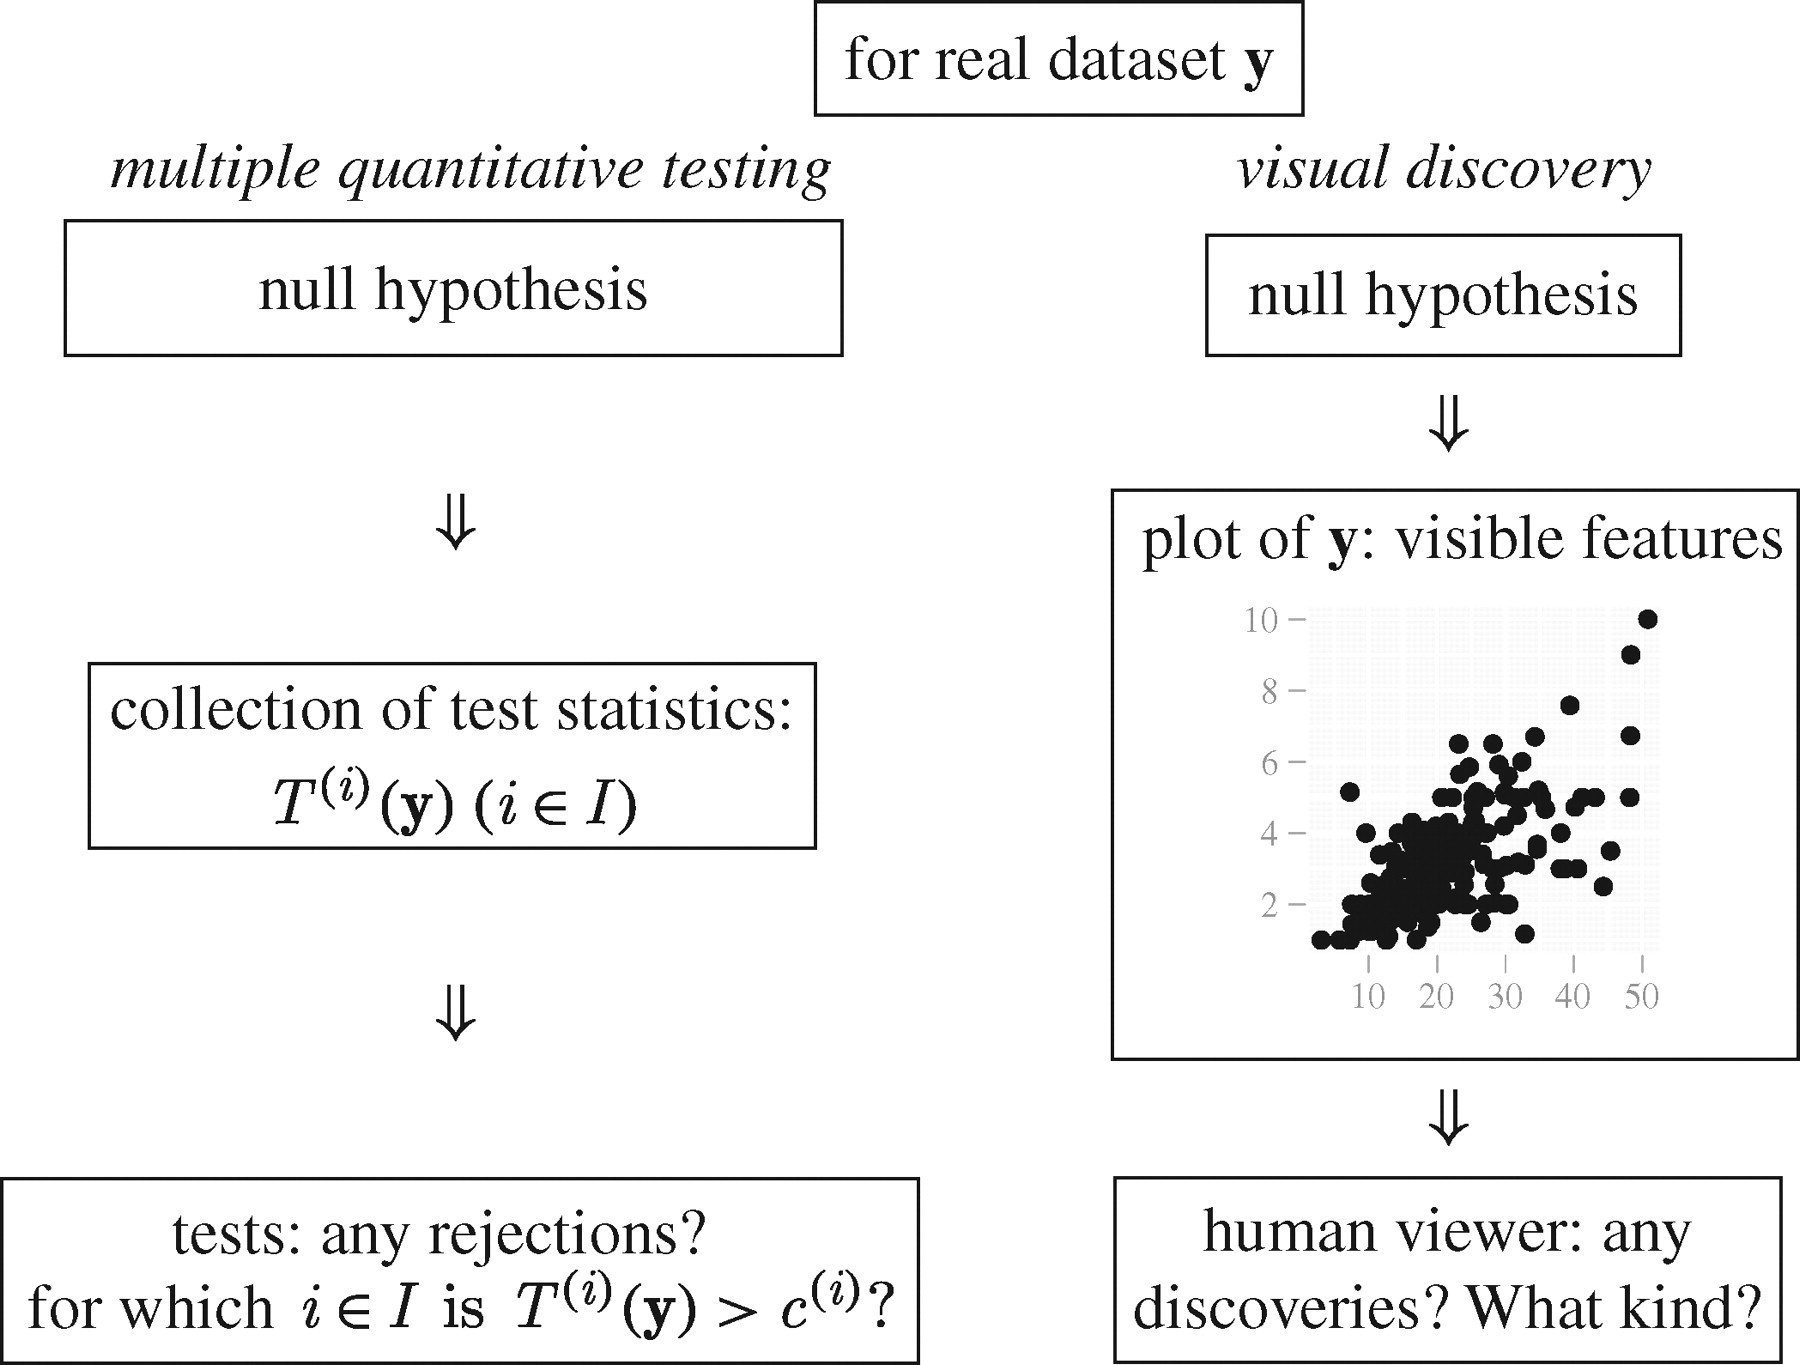
\includegraphics[width=4.6875in,height=3.55208in]{figures/rsta2009012001.jpg}
\caption{Parallelism between multiple quantitative testing and visual discovery \autocite{buja_statistical_2009}. Visible features in a plot are viewed as a collection of test statistics \(T^{(i)}(\boldsymbol{\mathrm{y}})~(i \in I)\), and any visual discoveries that are inconsistent with the null hypothesis are treated as evidence against the null. For model diagnostics, the null hypothesis would be the assumed model, and visual discoveries could be any visual features in favour of any alternatives. \label{fig:parallelism}}
\end{figure}



In visual inference, a visual discovery is defined as a rejection of a null hypothesis, and the same null hypothesis can be rejected by many different visual discoveries \autocite{buja_statistical_2009}. For model diagnostics, the null hypothesis would be the assumed model, while the visual discoveries would be any findings that are inconsistent with the null hypothesis. The same assumed model, such as classical linear regression model, can be rejected by many reasons with residual plot, including nonlinearity and heteroskedasticity as shown in Figure \ref{fig:residual-plot-cubic-heter}.

\begin{figure}
\centering
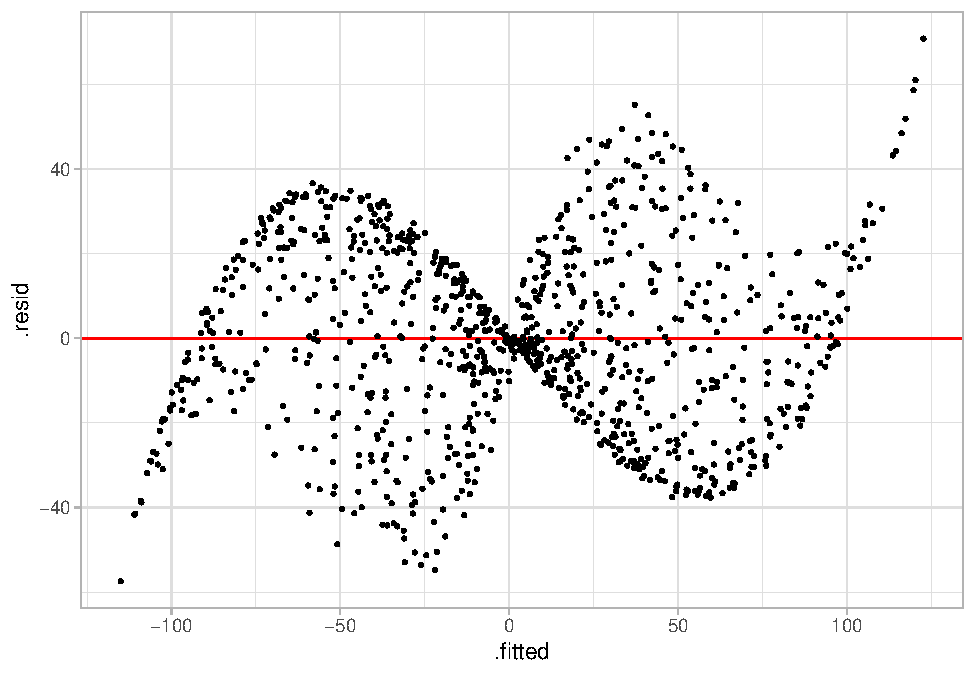
\includegraphics{thesis_files/figure-latex/residual-plot-cubic-heter-1.pdf}
\caption{\label{fig:residual-plot-cubic-heter}Residuals vs.~fitted values plot for a classical linear regression model. The residuals are produced by fitting a two-predictor multiple linear regression model with data generated from a cubic linear model. From the residual plot, ``butterfly shape'' can be observed which generally would be interpretd as evidence of heteroskedasticity. Further, from the outline of the shape, nonlinear patterns exist. Both visual discoveries are evidence against the null hypothesis, though heteroskedasticity actually does not exist in the data generating process.}
\end{figure}

\hypertarget{se:prespecification}{%
\section{Pre-specification of Visual Discoverable Features}\label{se:prespecification}}

As discussed in \textcite{buja_statistical_2009}, in the practice of model diagnostics, the range of possible visual discoveries is not pre-specified. In other words, people do not explicitly specify which visual feature(s) they are looking for before the reading the diagnostic plot. In contrary, conventional hypothesis testing always requires the pre-specification of the parameter space \(\Theta\) of the parameter of interest \(\theta \in \Theta\) to form a valid inferential procedure. To address this issue, a collection of test statistics \(T^{(i)}(\boldsymbol{\mathrm{y}})~(i \in I)\) is defined, where \(\boldsymbol{\mathrm{y}}\) is the data and \(I\) is a set of all possible visual features. \textcite{buja_statistical_2009} described each of the test statistics \(T^{(i)}(\boldsymbol{\mathrm{y}})\) as a measurement of the degree of presence of a visual feature. Alternatively, \textcite{majumder_validation_2013} avoids the use of visual features and defined the visual statistics \(T(.)\) as a mapping from a dataset to a data plot. Both definitions of visual test statistics are valid, but in the rest of the report the first definition will be used as it covers some details needed by the following discussion.

The size of the collection \(T^{(i)}(\boldsymbol{\mathrm{y}})~(i \in I)\) depends on the size of the set \(I\). Thus, if one can define \(I\) comprehensively, i.e, pre-specify all the visual discoverable features, the validity issue will be solved. Unfortunately, to our knowledge, there is no such a way to list all visual features. In linear regression diagnostics, possible visual features of a residual plot may be outliers, shapes and clusters. But this is an incomplete list which does not enumerate all the visual features.

Similarly, \textcite{wilkinson_graph-theoretic_2005} proposed the work called graph theoretic scagnostics, which adopted the idea of ``scagnostics'' - scatter plot diagnostics from (can't find the 1984 citation). It includes 9 computable scagnostics measures defined on planar proximity graphs: ``Outlying'', ``Convex'', ``Skinny'', ``Stringy'', ``Straight'', ``Monotonic'', ``Skewed'', ``Clumpy'' and ``Striated'' which attempts to describe outliers, shape, density, trend and coherence of the data. This approach is inspiring but it still does not give the complete list of visual discoverable features. In fact, it is possible that such a list will never be complete as suggested in \textcite{buja_statistical_2009}.

Thinking out of the box, \textcite{buja_statistical_2009} argued that there is actually no need for pre-specification of visual discoverable features. In model diagnostics, when the null hypothesis is rejected, the reasons for rejecting the hypothesis will also be known. This is because observers can not only point out the fact that visual discoveries have been found, but also describe the particular visual features they observed. Those features will correspond to the subset of the collection of visual test statistics \(T^{(i)}(\boldsymbol{\mathrm{y}})~(i \in I)\) which resulted in rejection. This argument helps justifies the validity of visual inference.

\hypertarget{se:sampling-from-null}{%
\section{Sampling from the Null Distribution}\label{se:sampling-from-null}}

In visual inference, the null distribution of plots refers to the infinite collection of plots of null datasets sampled from \(H_0\). It is defined as the analogue of the null distribution of test statistics in conventional test \autocite{buja_statistical_2009}. In practice, a finite number of plots of null datasets could be generated, called null plots.

In the context of model diagnostics, sampling data from \(H_0\) is equivalent to sampling data from the assumed model. As \textcite{buja_statistical_2009} suggested, \(H_0\) is usually composited by a collection of distributions controlled by nuisance parameters. Since statistical models can have various forms, there is no general solution to this problem, but it sometimes can be reduced to so called ``reference distribution'' by applying one of the three methods: (i) sampling from a conditional distribution given a minimimal sufficient statistic under \(H_0\), (ii) parametric bootstrap sampling with nuisance parameters estimated under \(H_0\), and (iii) Bayesian posterior predictive sampling.

The conditional distribution given a minimal sufficient statistic is the best justified reference distribution among the three \autocite{buja_statistical_2009}. Suppose there exists a minimal sufficient statistic \(\boldsymbol{S}(\boldsymbol{y})\) under the null hypothesis, any null datasets \(\boldsymbol{y^{*}}\) should fulfil the condition \(\boldsymbol{S}(\boldsymbol{y}) = \boldsymbol{s}\). Using the classical linear regression model as example, the minimal sufficient statistic is \(\boldsymbol{S}(\boldsymbol{y}) = (\hat{\boldsymbol{\beta}}, \boldsymbol{e}'\boldsymbol{e})\), where \(\hat{\boldsymbol{\beta}}\) are the coefficient estimators and \(\boldsymbol{e}'\boldsymbol{e}\) is the residual sum of square. Alternatively, the minimal sufficient statistic can be constructed as \(\boldsymbol{S}(\boldsymbol{y}) = (\hat{\boldsymbol{y}}, ||\boldsymbol{e}||)\), where \(\hat{\boldsymbol{y}}\) are the fitted values and \(||\boldsymbol{e}||\) is the length of residuals, which is more intuitive as suggested by \textcite{buja_statistical_2009}. Since the fitted values are held fixed, the variation can only occur in the residual space. And because the length of residual is also held fixed, residuals obtained from a null dataset has to be a random rotation of \(\boldsymbol{e}\) in the residual space. With this property, null residuals can be simulated by regressing \(N\) i.i.d standard normal random draws on the regressors, then rescaling it by the ratio of residual sum of square in two regressions.

\hypertarget{se:lineup}{%
\section{Lineup Protocol}\label{se:lineup}}

With the validity of visual inference being justified and the simulation of null plots being provided, another aspect of hypothesis testing that needs to be addressed is the control of false positive rate or Type I error. Any visual statistic \(T^{(i)}(\boldsymbol{\mathrm{y}})\) needs to pair with a critical value \(c^{(i)}\) to form a hypothesis test. When a visual feature \(i\) is discovered by the observer from a plot, the corresponding visual statistic \(T^{(i)}(\boldsymbol{\mathrm{y}})\) may not be known as there is no general agreement on the measurement of the degree of presence of a visual feature. It is only the event that \(T^{(i)}(\boldsymbol{\mathrm{y}}) > c^{(i)}\) is confirmed. Similarly, if any visual discovery is found by the observer, we say, there exists \(i \in I:~T^{(i)}(\boldsymbol{\mathrm{y}}) > c^{(i)}\) \autocite{buja_statistical_2009}.

Using the above definition, the family-wise Type I error can be controlled if one can provide the collection of critical values \(c^{(i)}~(i \in I)\) such that \(P(\mathrm{there~exists~} i \in I: T^{(i)}(\boldsymbol{\mathrm{y}}) > c^{(i)}|\boldsymbol{\mathrm{y}}) \leq \alpha\), where \(\alpha\) is the significance level. However, since the quantity of \(T^{(i)}(\boldsymbol{\mathrm{y}})\) may not be known, such collection of critical values can not be provided.

\textcite{buja_statistical_2009} proposed the lineup protocol as a visual test to calibrate the Type I error issue without the specification of \(c^{(i)}~(i \in I)\). It is inspired by the ``police lineup'' or ``identity parade'' which is the act of asking the eyewitness to identify criminal suspect from a group of irrelevant people. The protocol consists of \(m\) randomly placed plots, where one plot is the actual data plot, and the remaining \(m - 1\) plots have the identical graphical production as the data plot except the data has been replaced with data consistent with the null hypothesis. Then, an observer who have not seen the actual data plot will be asked to point out the most different plot from the lineup.

Under the null hypothesis, it is expected that the actual data plot would have no distinguishable difference with the null plots, and the probability of the observer correctly picks the actual data plot is \(1/m\). If we reject the null hypothesis as the observer correctly picks the actual data plot, then the Type I error of this test is \(1/m\).

This provides us with an mechanism to control the Type I error, because \(m\) - the number of plots in a lineup can be chosen. A larger value of \(m\) will result in a smaller Type I error, but the limit to the value of \(m\) depends on the number of plots a human is willing to view \autocite{buja_statistical_2009}. Typically, \(m\) will be set to \(20\) which is equivalent to set \(\alpha = 0.05\), a general choice of significance level for conventional testing among statisticians.

Further, if we involve \(K\) independent observers in a visual test, and let \(X\) be a random variable denoting the number of observers correctly picking the actual data plot. Then, under the null hypothesis \(X \sim \mathrm{Binom}_{K,1/m}\), and therefore, the \(p\)-value of a lineup of size \(m\) evaluated by \(K\) observer is given as
\begin{equation} \label{eq:pvaluesingle}
P(X \geq x) = \sum_{i=x}^{K}{{K}\choose{i}}\left(\frac{1}{m}\right)^i\left(\frac{m-1}{m}\right)^{k-i},
\end{equation}

where \(x\) is the realization of number of observers correctly picking the actual data plot \autocite{majumder_validation_2013}.

The multiple individuals approach avoids the limit of \(m\), while provides visual tests with \(p\)-value much smaller than \(0.05\). In fact, the lower bound of \(p\)-value decreases exponentially as \(K\) increases. With just \(4\) individuals and \(20\) data plots in a lineup, the \(p\)-value could be as small as \(0.0001\). Additionally, by involving multiple observers, variation of individual ability to read plots can be addressed to some degree as different opinions about visual discoveries can be collected.

Compared to the conventional test, whose power only depends on the parameter of interest \(\theta\), several studies \autocites[see][]{hofmann_graphical_2012,majumder_validation_2013,majumder_human_2014,roy_chowdhury_using_2015,loy_variations_2016} have shown the power of the visual test is subject-specific. Thus, to be able to account for individual's ability, an individual is required to evaluate multiple lineups \autocite{majumder_validation_2013}.

Suppose individuals have the same ability and a lineup has been evaluated by multiple individuals, under the alternative hypothesis, the estimated power for a lineup can be expressed as \(\hat{p} = x/K\), the estimated probability of identifying the actual data plot from the lineup. If the individual skill needs to be taken into account, and \(L\) lineups have been evaluated by \(K\) individuals, \textcite{majumder_validation_2013} suggests that mixed effects logistic regression model can be fit as:

\[g(p_{li}) = W_{li}\delta + Z_{li}\tau_{li},\]
where \(g(.)\) is the logit link function \(g(p) = log(p) - log(1-p)\); \(0 \leq p \leq 1\). \(W_{li}\), \(1 \leq i \leq K\), \(1 \leq l \leq L\), is the covariate matrix including lineup-specific elements and demographic information of individuals, and \(\delta\) is a vector of parameters. \(Z\) is the random effects matrix, and \(\tau\) is a vector of variables follow \(N(\boldsymbol{0},\sigma_{\tau}\boldsymbol{I}_{KL\times KL})\).

Then, the estimated power for lineup \(l\) and individual \(i\) can be calculated as \(\hat{p}_{li} = g^{-1}(W_{li}\hat{\delta} + Z_{li}\hat{\tau}_{li})\) \autocite{majumder_validation_2013}.

\hypertarget{se:limitation}{%
\section{Limitations of Lineup Protocol and Automatic Visual Inference}\label{se:limitation}}

Although lineup protocol has already been integrated into data analysis of various topics, such as diagnostics of hierarchical linear models \autocite{loy_diagnostic_2013}, geographical Research \autocite{widen_graphical_2016} and forensic examinations \autocite{krishnan_hierarchical_2021}, the involvement with human judgements limits its popularity. Similar to handicraft in pre-industrial society, lineup protocol conducted by humans is infeasible on a large scale, high in labour cost and time consuming. Moreover, it is strongly unfriendly to vision-impaired people.

The ``steam engine'' of visual inference needs to be developed for relieving people's workload by automating repeating tasks and providing standard result in a control environment. Large-scale evaluation of visual tests is not possible without the use of technology and machines.

Modern computer vision model could be a promising solution to this problem. As a subfield of AI, computer vision with the modern deep learning architectures solved numerous critical problems in automation. Inspired by the vision processing in living organisms, the convolutional neural network was introduced by \textcite{fukushima_neocognitron_1982}. Soon, this architecture was applied to hand-written number recognition trained with back-propagation by \textcite{lecun_backpropagation_1989}. This was one of the earliest attempts which human successfully extract information from digital images via self-learning algorithms. Modern computer vision model is typically built on the deep neural network with convolutional layers \autocite{fukushima_neocognitron_1982}. Convolutional layers take advantage of the hierarchical pattern in data and provide regularized versions of fully-connected layers. It downscales and transforms the image by summarising information in a small space. Numerous studies have shown that it can be used to effectively tackle vision tasks, such as image recognition \autocite{rawat_deep_2017}. With the development of graphics processing units and the spread of high-performance personal computers, researches in computer vision become a new hype in the 21st century. Achievements such as computer-aided diagnosis \autocite{lee_image_2015}, pedestrian detection \autocite{brunetti_computer_2018} and facial recognition \autocite{emami_facial_2012} had a significant impact on our daily life.

Using computer vision models to read data plots is not a general choice. some fields have adopted this idea by applying computer vision models to read recurrence plots for time series regression \autocite{ojeda_multivariate_2020}, time series classification \autocite{chu_automatic_2019,hailesilassie_financial_2019,hatami_classification_2018,zhang_encoding_2020}, anomaly detection \autocite{chen_convolutional_2020} and pairwise causality analysis \autocite{singh_deep_2017}. However, evaluating lineups with computer vision model is a new field of study.

\hypertarget{research-problem}{%
\chapter{Research Problem}\label{research-problem}}

The main objective of this research is to build an automatic visual inference system for the purpose of conducting large-scale visual test. The research will focus on three projects as follows:

\begin{enumerate}
\def\labelenumi{\arabic{enumi}.}
\item
  Develop a prototype of automatic visual inference system for evaluating lineups of residual plots of the classical normal linear regression model and study factors that affect the performance of the system with comparison to human subjects.
\item
  Extend and enhance the automatic visual inference system developed in the first project to general lineup protocol problems by adopting image similarity assessed by computer vision models.
\item
  Validate and apply the automatic visual inference system to predictive model diagnostics on empirical data.
\end{enumerate}

\hypertarget{overview-of-the-thesis}{%
\chapter{Overview of the Thesis}\label{overview-of-the-thesis}}

The first project develops a prototype of automatic visual inference system for evaluating lineups of residual plots, with a focus on the classical normal linear regression model given it is one of the simplest predictive models. The automatic system is identical to the lineup protocol except evaluators are replaced by computer vision models. The computer vision models are trained by using data simulated from linear models with violations of different classical assumptions, such as linearity and homoscedasticity. Data of human performance on evaluating residual plots generated under the same simulation setting is collected by conducting online human subject experiments, such that the comparison between the power of human subject-assessed visual tests and the system-assessed visual tests can be made. Finally, factors that affect the performance of the automatic system are studied for improving the architecture and design of the computer vision models.

The second project aims to extend the automatic system to lineup protocol with no assumptions on the type of the data plot and the data generating process. It only requires the protocol to asks the evaluators to select the most different plot(s) from the lineup. The automatic system will be built upon image similarity produced by computer vision models.

The third project aims to apply the automatic system to predictive model diagnostics on empirical data. Potential predictive models considered by this research are linear model, generalized linear models and non-parametric regression. Multiple human subject experiments will need to be conducted to validate the effectiveness of the automatic system.

\hypertarget{automatic-visual-statistical-inference-for-linear-regression-diagnostics}{%
\chapter{Automatic Visual Statistical Inference for linear regression diagnostics}\label{automatic-visual-statistical-inference-for-linear-regression-diagnostics}}

This project focuses on building a prototype of automatic visual statistical inference system for evaluating residual plots of classical normal linear regression model. To set up a comparison between the computer vision models and humans, human subject experiments were conducted to understand the ability of human reading residual plots.

Because the first project is still ongoing, we consider the result we have is not enough to write as a paper at the moment. Hence, the material provided in this section is two main parts of the draft paper that will contain enough details for understanding the project.

\hypertarget{human-subject-exeriments}{%
\section{Human Subject Exeriments}\label{human-subject-exeriments}}

To collect data of human performance on reading residual plot of linear regression model with nonlinearity and heteroskedasticity defects, two human experiments were conducted. Participants of both experiments were recruited using an online platform called Prolific \autocite{prolific_prolific_2022}.

Prolific provides an international participant pool with the option to apply flexible pre-screening filters. In this study, we recruited \(62\) participants who was fluent in English with at least \(10\) previous submissions and \(98\)\% approval rate in other Prolific studies for quality control. Further, balance sample across gender was imposed to prevent gender bias.

In Prolific, researchers can either approve or reject submissions based on the quality of the responses. If a submission is approved by the researcher, the participant will be paid a certain amount of money per hour of time spent on the experiment. To assess the quality of the responses, two attention checks were given to each participant during the experiment, where at least one of them was required to pass for the approval of submission.

Throughout the experiments, participants were requested to complete a short survey and evaluate 20 lineups on a website in an hour. Each lineup consists of one actual residual plot and 19 null residual plots produced by plotting null residuals simulated from the residual rotation distributions. Among the 20 lineups, there were two extremely easy lineups used as attention checks which everyone should get correct. The short survey was intended to collect information about participant that might affect their ability in reading data plot including age, highest level of education, preferred pronoun and previous experience in similar study. For the evaluation of the lineup, participant first needed to select one or multiple most different data plot(s) from the lineup by clicking the corresponding image. Then, the primary reason for choosing the plots needed to be provided by picking one of the given options - ``outlier(s)'', ``cluster(s)'', ``shape'' and ``other''. Explanations about these options were provided in the training page and the mouseover text. Table \ref{tab:lineup-reason} gives the detailed explanations about these reasons. If the option ``other'' was selected, text input for the specified reason would be collected. Lastly, the degree of difference between their chosen data plot(s) and other data plots needed to be selected among five levels - ``not at all'', ``slightly'', ``moderately'', ``very'' and ``extremely''. Notably, if participants could not tell the difference between the data plots, there was an option to skip the evaluation of the lineup. However, to prevent participants abusing this option, warnings were given at the beginning of the study that skipping too many lineups might lead to rejection of submission since it demonstrated clear low-effort throughout the experiment.

\begin{table}

\caption{\label{tab:lineup-reason}Explanations about reasons for choosing data plots from a lineup}
\centering
\resizebox{\linewidth}{!}{
\begin{tabular}[t]{ll}
\toprule
Reasons & Explanations\\
\midrule
outlier(s) & In a data plot, an outlier is a point that differs significantly from other points.\\
cluster(s) & In a data plot, a cluster is a group of points positioned closely together. 
And usually, there will be gaps between different clusters.\\
shape & It could be any common shapes we would see in real life, like triangle shape, U-shape, butterfly shape, etc.\\
other & Patricipants needs to give their reasons in the text input.\\
\bottomrule
\end{tabular}}
\end{table}

The study website was powered by Flask \autocite{grinberg_flask_2018}, a web framework written in Python 3 \autocite{van_rossum_python_2009}, hosted on PythonAnywhere \autocite{pythonanywhere_pythonanywhere_2022}, a web hosting service provider. Due to the limit of the storage on PythonAnywhere, lineup images needed for the website were hosted separately on Github Pages \autocite{gtihub_github_2022-1}, a static site hosting service provided by Github \autocite{gtihub_github_2022}, stored in private Github repositories. The uniform resource locator (URL) to lineup images were set to be unique random strings such that images can not be accessed by general approaches without knowing the correct URL. This avoided participants seeing the lineup beforehand. The front-end of the website was built using a JavaScript \autocite{flanagan_javascript_2006} library jsPsych \autocite{de_leeuw_jspsych_2015} which is specialized in creating online behavioral experiments. One of the reasons we chose to use this library was it had a modularized but highly customizable template which could record participant's response time automatically. This is essential for us to confirm the quality of the data by checking exceptionally fast or slow responses. Figure \ref{fig:diagram-experiment} summarizes the online experiment setup.

\begin{figure}
\centering
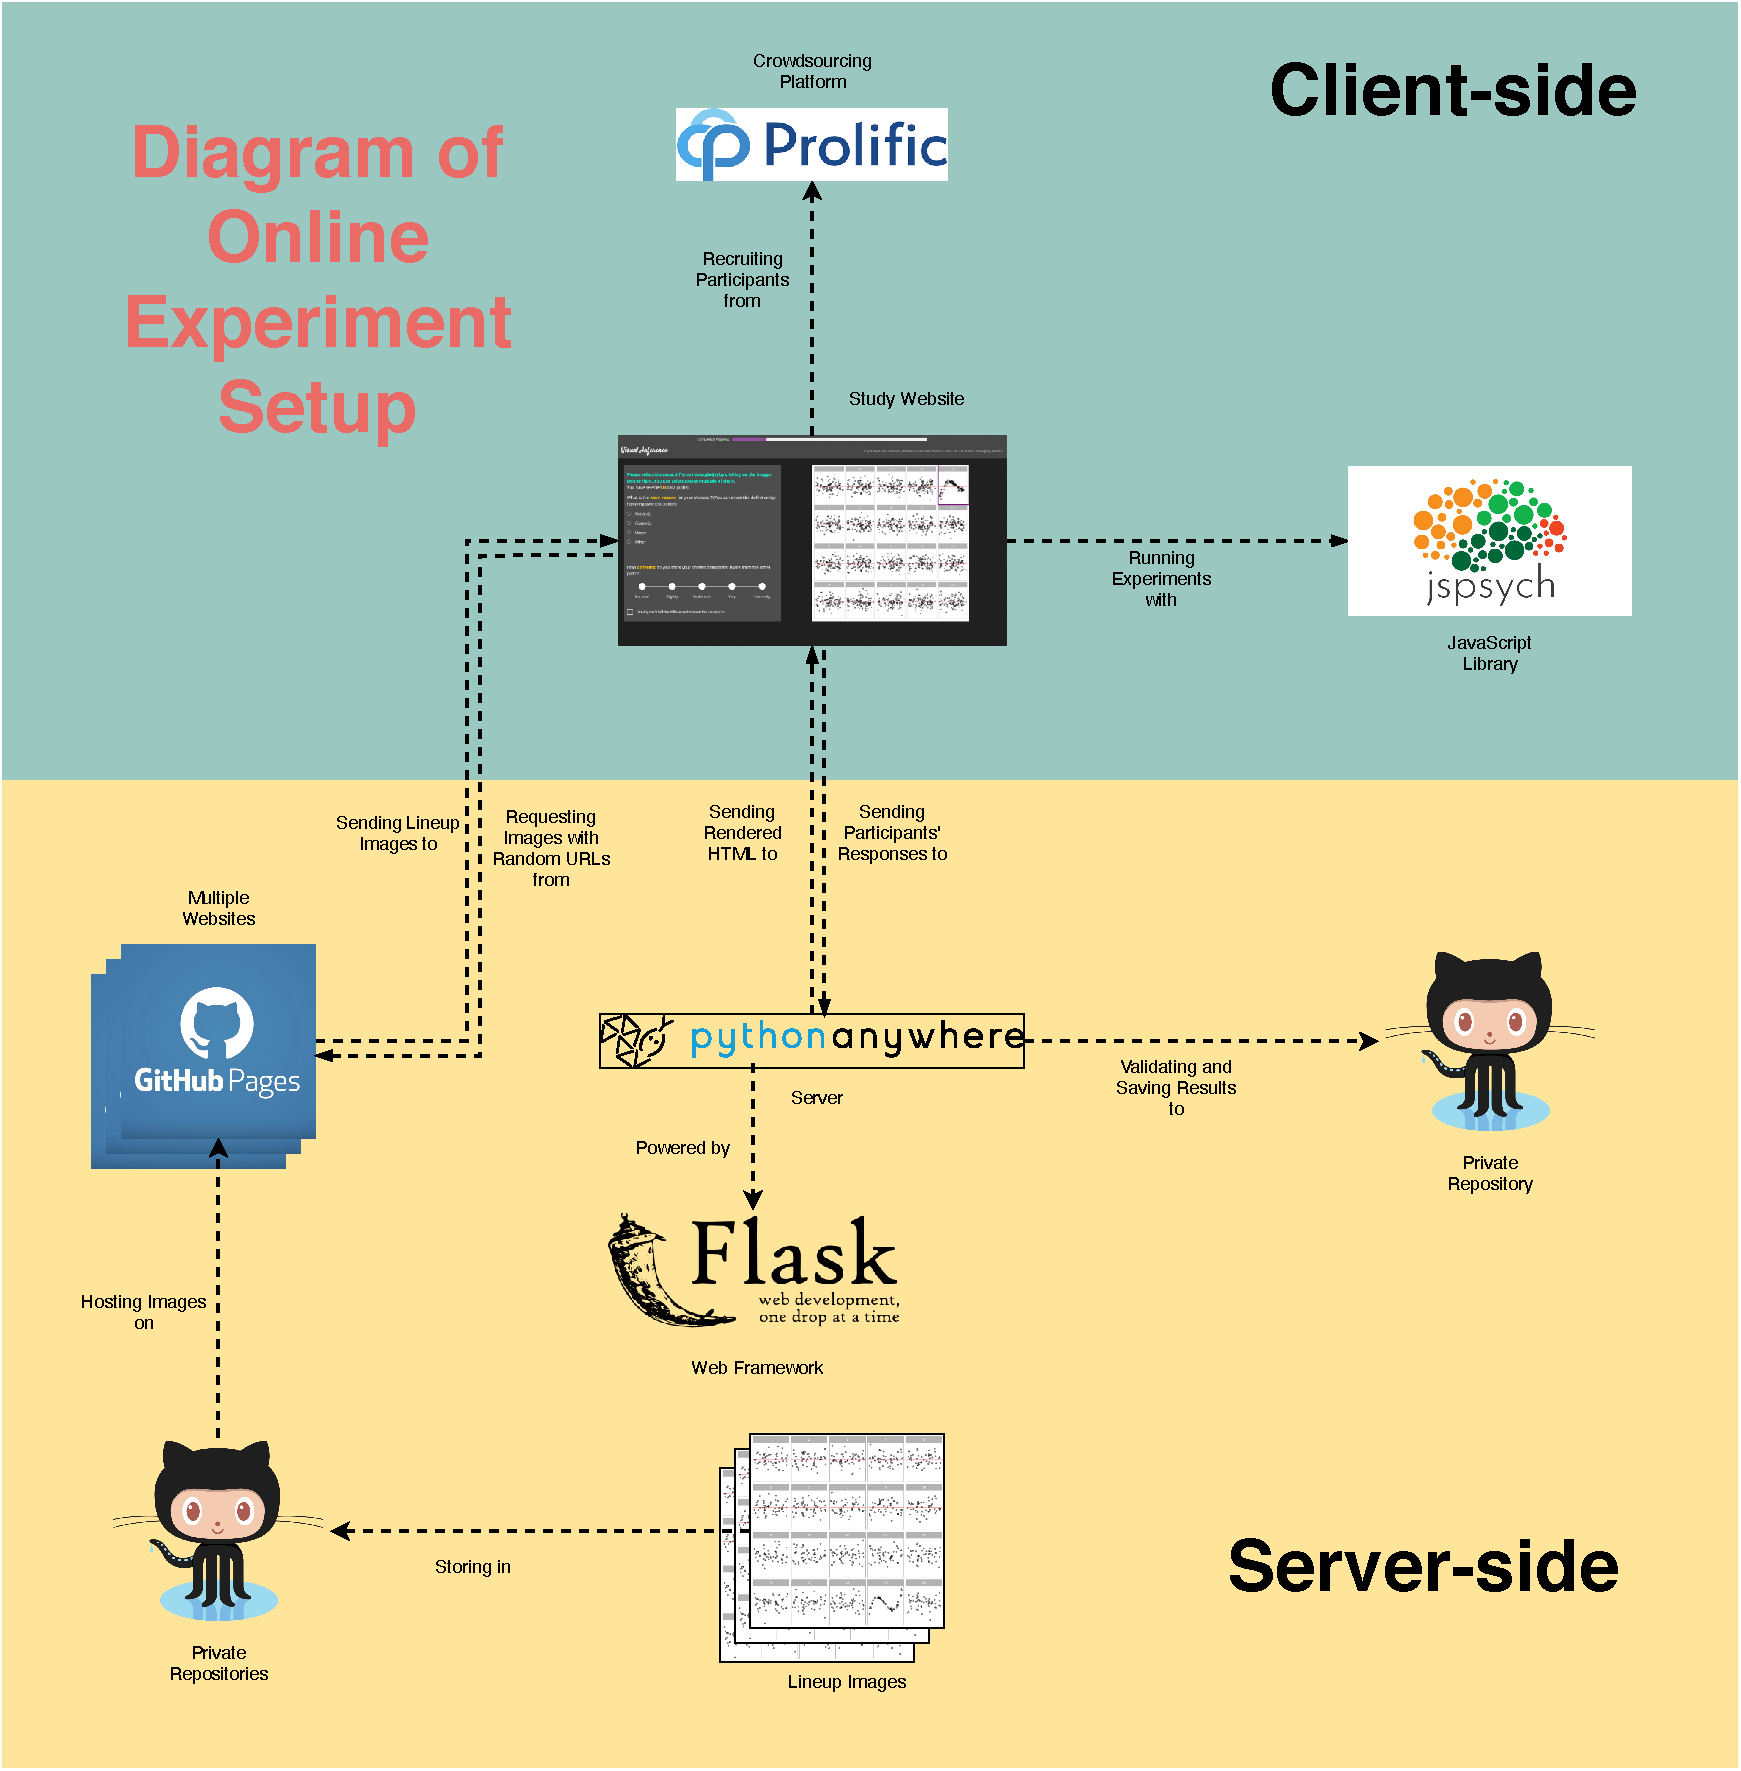
\includegraphics[width=4.6875in,height=4.6875in]{figures/experiment_tech.pdf}
\caption{Diagram of online experiment setup. The server-side of the study webiste used Flask as backend hosted on PythonAnywhere. And the client-side used jsPsych to run experiment. \label{fig:diagram-experiment}}
\end{figure}

The first two pages of the website are the explanatory statement and the consent form. Participants were asked to read the documents and agree with the terms to advance to the short survey. With the completion of the survey, the next page is the training page, which contained instructions on how to interact with the webpage. Followed by the training page, there are 20 lineups each on a single page. Figure \ref{fig:website-layout} illustrates the layout of the website. At the end of the experiment, participants would be redirected back to Prolific and waited for researchers' responses.

\begin{figure}
\centering
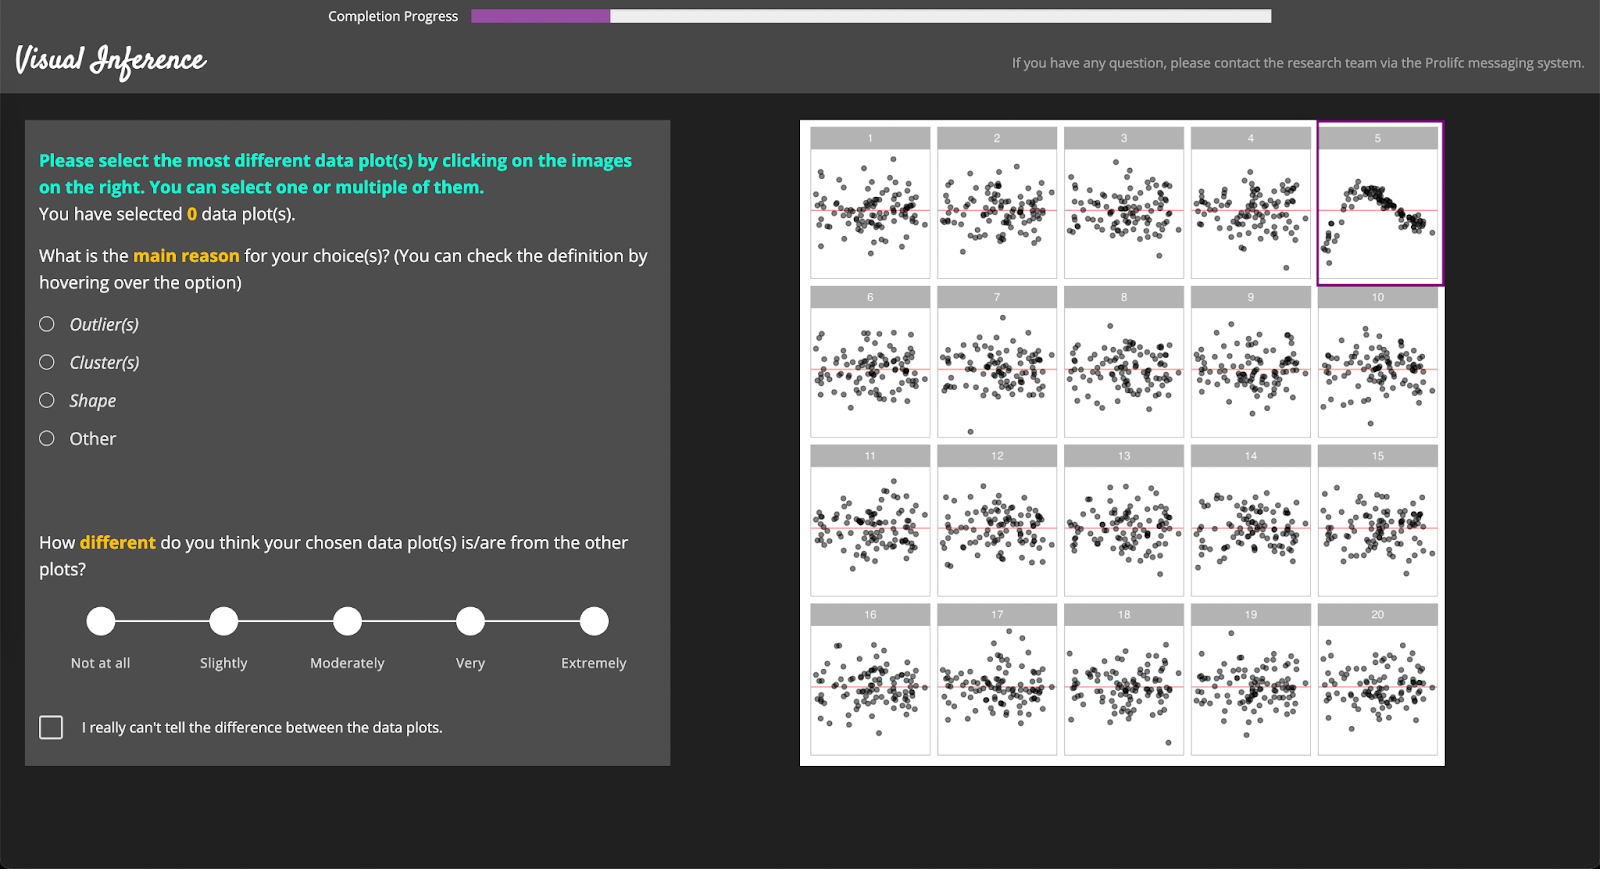
\includegraphics[width=5.72917in,height=3.11458in]{figures/website.png}
\caption{Layout of the study website. Participants needed to choose the most different plots on the right and select their reasons and confidence levels on the left. \label{fig:website-layout}}
\end{figure}

Next we will discuss the simulation setup for this study. The experiment data was simulated by the use of the programming language \texttt{R} \autocite{r_core_team_r_2021}. For the ease of reproducibility, functions to build models, simulate data from models, produce lineup with data, allocate stimulis for subjects and evaluate subject responses from this study are bundled in the package \texttt{visage} with a unique object-oriented programming system built upon the environment feature of \texttt{R}. In the description of the simulation, corresponding functionalities of the package will be introduced.

Two models were used in the study, where both were linear models with some degree of violations of classical assumptions.

\hypertarget{cubic-model}{%
\subsection{Cubic Model}\label{cubic-model}}

The first model was a cubic linear model with two regressors, which can be expressed by:
\begin{equation} \label{eq:cubic}
\boldsymbol{Y}= 1 + (2-c)\boldsymbol{X} + c\boldsymbol{Z} + a[(2-c)\boldsymbol{X}]^2+a(c\boldsymbol{Z})^2+b[(2-c)\boldsymbol{X}]^3+b(c\boldsymbol{Z})^3+\boldsymbol{\varepsilon},
\end{equation}
where \(c \in (0,2)\), \(a \in (-3,3)\), \(b \in (-3,3)\), \(\boldsymbol{\varepsilon}\overset{iid}{\sim} N(\boldsymbol{0},\sigma^2\boldsymbol{I})\), \(\boldsymbol{Y}\), \(\boldsymbol{X}\) and \(\boldsymbol{Z}\) are \(n\times1\) matrices.

This defines a cubic relationship between \(\boldsymbol{Y}\), \(\boldsymbol{X}\) and \(\boldsymbol{Z}\). Meanwhile, to create nonlinearity defect, the null model followed the assumptions of the classical normal linear regression model (CNLRM), fitted by OLS is:
\begin{equation} \label{eq:cubic_null}
\boldsymbol{Y}=\beta_0+\beta_1\boldsymbol{X}+\beta_2\boldsymbol{Z}+\boldsymbol{u},
\end{equation}
where \(\boldsymbol{u} \sim N(0,\sigma^2_u\boldsymbol{I})\).

Clearly, omitted-variable bias will present since the null model leaves out the quadric and cubic terms.

\begin{lemma}[Distribution of residuals produced by the cubic model] \label{lemma:cubic}
Given the data generating process in Equation (\ref{eq:cubic}), and null model in Equation (\ref{eq:cubic_null}). Let $\boldsymbol{X}_a=[\boldsymbol{1},\boldsymbol{X},\boldsymbol{Z}]$ denotes the set of regressors in matrix form. Then, the residuals obtained from the null model are $$\boldsymbol{e} \sim N(\boldsymbol{R}_a\boldsymbol{X}_b\boldsymbol{\beta}_b, \sigma^2\boldsymbol{R}_a),$$ where $\boldsymbol{R}_a=\boldsymbol{I}-\boldsymbol{X}_a(\boldsymbol{X}_a'\boldsymbol{X}_a)^{-1}\boldsymbol{X}_a'$, $\boldsymbol{X}_b=[\boldsymbol{X}^2,\boldsymbol{Z}^2,\boldsymbol{X}^3,\boldsymbol{Z}^3]$ and $\boldsymbol{\beta}_b=(a(2-c)^2,ac^2,b(2-c)^3,bc^3)'$.
\end{lemma}

\begin{proof}
Using the Frisch–Waugh–Lovell theorem, the residuals obtained by the null model are $$\boldsymbol{e}=\boldsymbol{R}_a\boldsymbol{Y}=\boldsymbol{R}_a(\boldsymbol{X}_a\boldsymbol{\beta}_a+\boldsymbol{X}_b\boldsymbol{\beta}_b+\boldsymbol{\varepsilon}),$$ where $\boldsymbol{R}_a=\boldsymbol{I}-\boldsymbol{X}_a(\boldsymbol{X}_a'\boldsymbol{X}_a)^{-1}\boldsymbol{X}_a'$, $\boldsymbol{\beta}_a=(1,2-c,c)'$, $\boldsymbol{X}_b=[\boldsymbol{X}^2,\boldsymbol{Z}^2,\boldsymbol{X}^3,\boldsymbol{Z}^3]$ and $\boldsymbol{\beta}_b=(a(2-c)^2,ac^2,b(2-c)^3,bc^3)'$. 

Because $\boldsymbol{R}_a\boldsymbol{X}_a=\boldsymbol{0}$, we have $\boldsymbol{e}=\boldsymbol{R}_a(\boldsymbol{X}_b\boldsymbol{\beta}_b+\boldsymbol{\varepsilon}).$ Since $\boldsymbol{\varepsilon} \sim N(0,\sigma^2\boldsymbol{I})$, it follows that $\boldsymbol{e} \sim N(\boldsymbol{R}_a\boldsymbol{X}_b\boldsymbol{\beta}_b, \sigma^2\boldsymbol{R}_a)$. 
\end{proof}

Lemma \ref{lemma:cubic} shows that the expectation of the residuals is clearly a function of \(\boldsymbol{X}\) and \(\boldsymbol{Z}\), which indicates the residuals and the fitted values \(\hat{Y} = \boldsymbol{X}_a(\boldsymbol{X}_a'\boldsymbol{X}_a)^{-1}\boldsymbol{X}_a'\boldsymbol{Y}\) are associated. Hence, it is expected that visual discoveries can be found in the residuals vs.~fitted values plot. Let \(X_i\) and \(Z_i\), \(i = 1,...,n\), be independent random variables follow uniform distribution \(U(-1,1)\). Given the expectation of the residuals, we could plot the expected values of residuals against the observed values. Figure \ref{fig:cubic-shape-1}, \ref{fig:cubic-shape-2} and \ref{fig:cubic-shape-3} illustrate the shape of residuals and their expected values under different parameter settings.

From the Figure \ref{fig:cubic-shape-1}, it can be observed that with fixed \(\sigma\) and \(c\), \(a\) and \(b\) are controlling the 2D projection of a hypersurface, and seemingly performing some rotations along different axes. Figure \ref{fig:cubic-shape-2} shows that with fixed \(a\), \(b\) and \(\sigma\), \(c\) is controlling the contribution of \(\boldsymbol{X}\) and \(\boldsymbol{Z}\) to \(\boldsymbol{Y}\). As \(c\) moves toward \(0\) or \(2\), one regressor will dominate another, which will mitigate some joint effects and resemble a typical cubic function. In Figure \ref{fig:cubic-shape-3}, \(a\), \(b\) and \(c\) are held fixed, and \(\sigma\) is controlling the noises around the expected values. The underlying shape is clearer for smaller \(\sigma\).

\begin{figure}
\centering
\includegraphics{thesis_files/figure-latex/cubic-shape-1-1.pdf}
\caption{\label{fig:cubic-shape-1}A matrix of residuals vs.~fitted values plot under different parameter settings of the cubic model. Resdiauls are drawns in black and the expected values are drawn in red. The plots show that if \(\sigma\) and \(c\) are held fixed, \(a\) and \(b\) rotate a two-dimension projection of a hypersurface.}
\end{figure}

\begin{figure}
\centering
\includegraphics{thesis_files/figure-latex/cubic-shape-2-1.pdf}
\caption{\label{fig:cubic-shape-2}A matrix of residuals vs.~fitted values plot under different parameter settings of the cubic model. Resdiauls are drawns in black and the expected values are drawn in red. The plots show that if \(a\), \(b\) and \(\sigma\) are held fixed, \(c\) controls the contribution of \(\boldsymbol{X}\) and \(\boldsymbol{Z}\) to \(\boldsymbol{Y}\).}
\end{figure}

\begin{figure}
\centering
\includegraphics{thesis_files/figure-latex/cubic-shape-3-1.pdf}
\caption{\label{fig:cubic-shape-3}A matrix of residuals vs.~fitted values plot under different parameter settings of the cubic model. Resdiauls are drawns in black and the expected values are drawn in red. The plots show that if \(a\), \(b\) and \(c\) are held fixed, \(\sigma\) controls the strength of the signal.}
\end{figure}

The residuals used in these three figures are simulated from the cubic models built using the \texttt{cubic\_model()} function from the package \texttt{visage}. \texttt{cubic\_model()} is a cubic model class constructor, which takes arguments \texttt{a}, \texttt{b}, \texttt{c}, \texttt{sigma}, \texttt{x} and \texttt{z}, where the first four are numeric values defined above, and \texttt{x} and \texttt{z} are random variable instances created by the random variable abstract base class constructor \texttt{rand\_var()}.

If we would like \(\boldsymbol{X}\) and \(\boldsymbol{Z}\) to be random uniform variables ranged from \(-1\) to \(1\), it can be achieved by using the random uniform variable class constructor \texttt{rand\_uniform()} inherited from the random variable abstract base class. It only takes two arguments which are the lower bound and the upper bound of the support.

\begin{Shaded}
\begin{Highlighting}[]
\FunctionTok{library}\NormalTok{(visage)}
\NormalTok{mod }\OtherTok{\textless{}{-}} \FunctionTok{cubic\_model}\NormalTok{(}\AttributeTok{a =} \SpecialCharTok{{-}}\DecValTok{3}\NormalTok{, }\AttributeTok{b =} \SpecialCharTok{{-}}\DecValTok{3}\NormalTok{, }\AttributeTok{c =} \DecValTok{1}\NormalTok{, }\AttributeTok{sigma =} \FloatTok{0.5}\NormalTok{, }
                   \AttributeTok{x =} \FunctionTok{rand\_uniform}\NormalTok{(}\SpecialCharTok{{-}}\DecValTok{1}\NormalTok{, }\DecValTok{1}\NormalTok{), }\AttributeTok{z =} \FunctionTok{rand\_uniform}\NormalTok{(}\SpecialCharTok{{-}}\DecValTok{1}\NormalTok{, }\DecValTok{1}\NormalTok{))}
\end{Highlighting}
\end{Shaded}

An instance of cubic model class contains methods of simulating data and making residual plot. Method \texttt{mod\$gen()} returns a data frame containing realizations of \(X\), \(Z\), \(Y\) and \(\varepsilon\) simulated from the model. The number of realizations depends on the integer argument \texttt{n}. In addition, if argument \texttt{fit\_model\ =\ TRUE}, a null model will be fitted using the simulated data and residuals and fitted values will be included in the returned data frame.

\begin{Shaded}
\begin{Highlighting}[]
\NormalTok{mod}\SpecialCharTok{$}\FunctionTok{gen}\NormalTok{(}\AttributeTok{n =} \DecValTok{5}\NormalTok{, }\AttributeTok{fit\_model =} \ConstantTok{TRUE}\NormalTok{)}
\end{Highlighting}
\end{Shaded}

\begin{verbatim}
##            y          x          z           e     .resid    .fitted
## 1 -0.8263671 -0.4988275  0.5569648 -0.06142887  1.2340651 -2.0604322
## 2  0.6134661  0.1762335  0.6512424  0.99654342  1.1758970 -0.5624310
## 3  0.2285071 -0.2814395 -0.1511556 -0.10996690 -0.3757603  0.6042674
## 4 -4.6320382 -0.5813456  0.9251409 -0.60826338 -1.2664307 -3.3656075
## 5  0.3148180  0.5647967  0.4406211  0.64596536 -0.7677711  1.0825892
\end{verbatim}

Method \texttt{mod\$plot()} produce a \texttt{ggplot} \autocite{wickham_ggplot2_2011} object. It takes a data frame containing columns \texttt{.resid} and \texttt{.fitted} as input, along with a character argument \texttt{type} indicating the type of the data plot, and other aesthetic arguments such as \texttt{size} and \texttt{alpha} to control the appearance of the plot.

\begin{Shaded}
\begin{Highlighting}[]
\NormalTok{mod}\SpecialCharTok{$}\FunctionTok{plot}\NormalTok{(mod}\SpecialCharTok{$}\FunctionTok{gen}\NormalTok{(}\AttributeTok{n =} \DecValTok{100}\NormalTok{, }\AttributeTok{fit\_model =} \ConstantTok{TRUE}\NormalTok{), }\AttributeTok{type =} \StringTok{"resid"}\NormalTok{, }\AttributeTok{size =} \DecValTok{1}\NormalTok{)}
\end{Highlighting}
\end{Shaded}

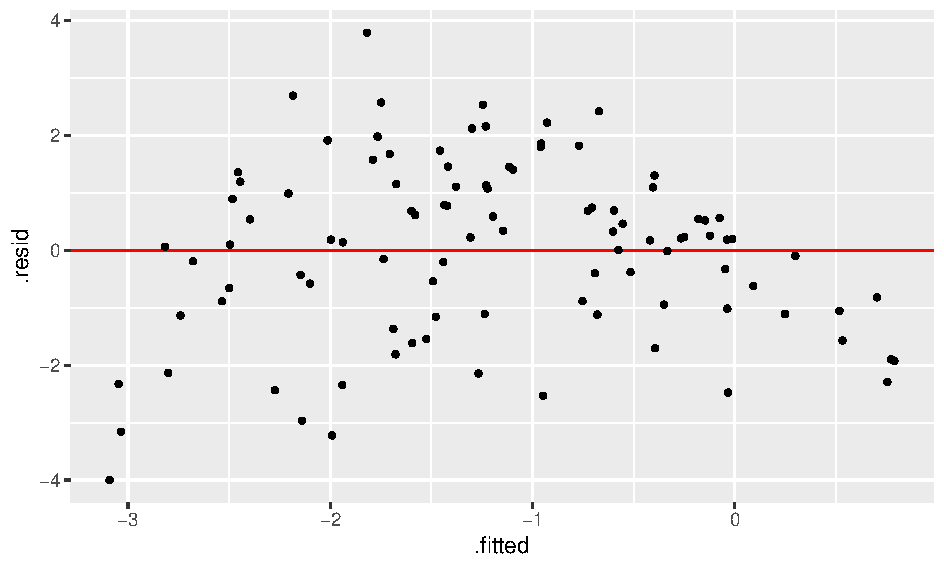
\includegraphics{thesis_files/figure-latex/test3-1.pdf}

Lineup is a matrix of residual plots which can be produced by using the methods \texttt{mod\$gen\_lineup()} and \texttt{mod\$plot\_lineup()}. Method \texttt{mod\$gen\_lineup} takes the number of realizations \texttt{n} and the number of plots in a lineup \texttt{k} as inputs. And the method \texttt{mod\$plot\_lineup()} has the same user interface as \texttt{mod\$plot()}.

\begin{Shaded}
\begin{Highlighting}[]
\NormalTok{mod}\SpecialCharTok{$}\FunctionTok{plot\_lineup}\NormalTok{(mod}\SpecialCharTok{$}\FunctionTok{gen\_lineup}\NormalTok{(}\AttributeTok{n =} \DecValTok{50}\NormalTok{, }\AttributeTok{k =} \DecValTok{20}\NormalTok{), }\AttributeTok{type =} \StringTok{"resid"}\NormalTok{, }\AttributeTok{size =} \DecValTok{1}\NormalTok{)}
\end{Highlighting}
\end{Shaded}

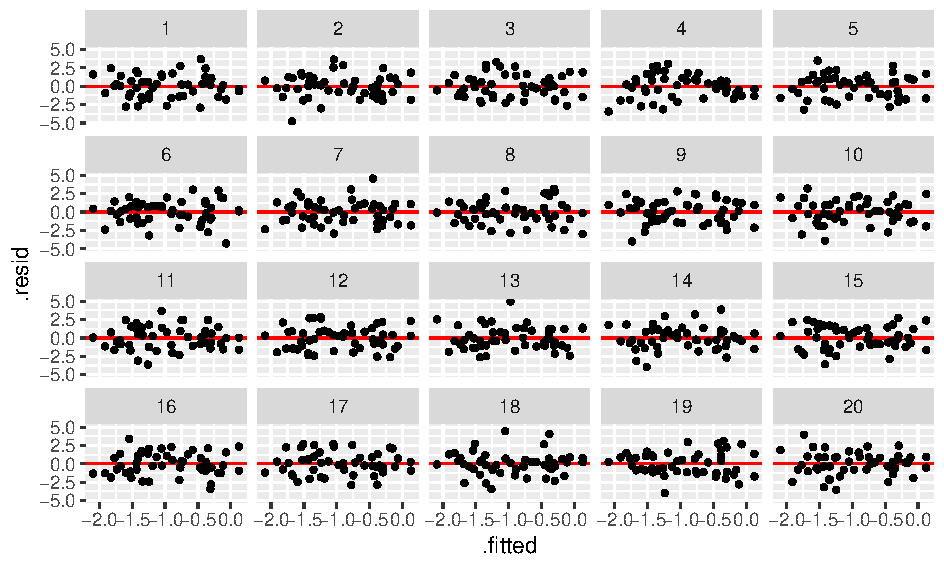
\includegraphics{thesis_files/figure-latex/unnamed-chunk-4-1.pdf}

The cubic model class also provides method to compute the expected values of residuals. Method \texttt{mod\$E()} takes a data frame with columns \texttt{x} and \texttt{z} as input, and returns a vector of expected values of residuals.

\begin{Shaded}
\begin{Highlighting}[]
\NormalTok{mod}\SpecialCharTok{$}\FunctionTok{E}\NormalTok{(mod}\SpecialCharTok{$}\FunctionTok{gen}\NormalTok{(}\AttributeTok{n =} \DecValTok{5}\NormalTok{))}
\end{Highlighting}
\end{Shaded}

\begin{verbatim}
## [1] -0.092183951 -0.003912092 -0.001531723  0.148353478 -0.050725712
\end{verbatim}

Since we know that under the null hypothesis, the residual \(\boldsymbol{e}\sim N(\boldsymbol{0},\sigma^2\boldsymbol{R}_a)\). Thus, the difference between the expected values \(\boldsymbol{R}_a\boldsymbol{X}_b\boldsymbol{\beta}_b\) and \(\boldsymbol{0}\) represents the direct impact of the parameters \(a\) and \(b\) on the residuals. It is expected that the larger the magnitude of the expected value relative to the variance and covariance, the easier the human to spot the patterns in the residual plot.

To obtain a measure of the impact of \(a\) and \(b\) on the residuals adjusted for variance and covariance, we need to address several properties of the residuals. First, the variance of the residuals \(\sigma^2\boldsymbol{R}_a\) is not an identity matrix. This can be fixed by standardizing the residuals by their variance-covariance matrix. Second, the difference between \(\boldsymbol{R}_a\boldsymbol{X}_b\boldsymbol{\beta}_b\) and \(\boldsymbol{0}\) could be negative, which is not ideal for comparison. Thus, the magnitude needs to be squared. Third, the measure needs to be a scalar. We could apply a weighted average operator \(\boldsymbol{W}\) on the transformed expected residuals to obtain a single numeric value. For simplicity, we set \(\boldsymbol{W}=n^{-1}\boldsymbol{1}\). Considering the high time complexity of computing the square root of \(\boldsymbol{R}_a\), off-diagonal elements of \(\boldsymbol{R}_a\) are set to be zeros. This gives the effect size: \[ES=n^{-1}||\sigma^{-1}\boldsymbol{R}_a^{-\frac{1}{2}}\boldsymbol{R}_a\boldsymbol{X}_b\boldsymbol{\beta}_b||^2=n^{-1}\sigma^{-2}||\boldsymbol{R}_a^{\frac{1}{2}}\boldsymbol{X}_b\boldsymbol{\beta}_b||^2\approx n^{-1}\sigma^{-2}||diag(\boldsymbol{R}_a)^{\frac{1}{2}}\boldsymbol{X}_b\boldsymbol{\beta}_b||^2,\] where \(diag(\boldsymbol{R}_a)\) is the diagonal matrix constructed from the diagonal elements of \(\boldsymbol{R}_a\).

The interpretation of this effect size is the impact of parameter \(a\) and \(b\) on the squared deviation of the standardized expected residual per observation. It is not directly related to the shape, or the pattern human observed from the residual plot, but it is a reasonable approximation of the degree of the visual deviation from the null residuals under our cubic model setting. Figure \ref{fig:effectsize} shows four residual plots with different effect sizes. As effect sizes increases, the strength of the signal become stronger.

\begin{figure}
\centering
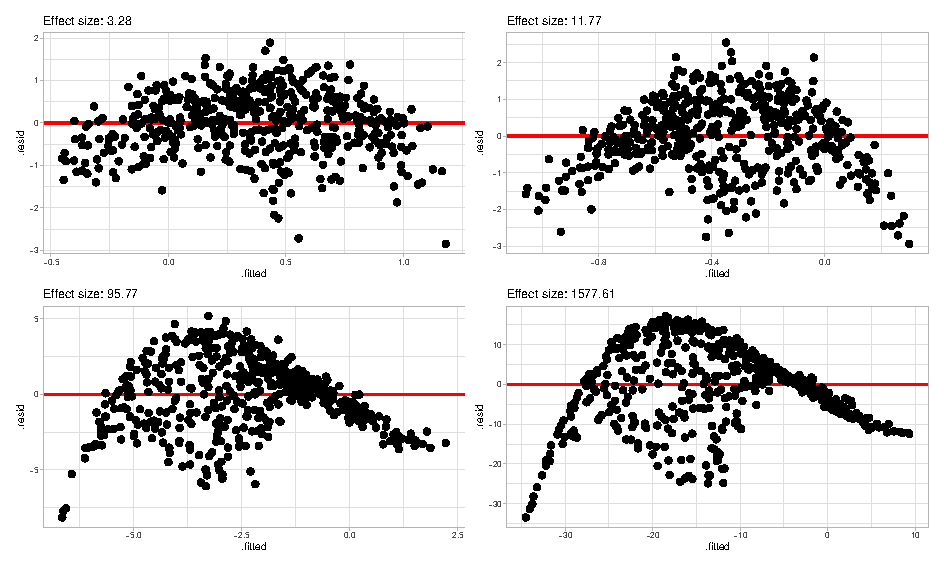
\includegraphics{thesis_files/figure-latex/effectsize-1.pdf}
\caption{\label{fig:effectsize}Cubic model residual plots under different effect sizes. The larger the effect size, the stronger the signal.}
\end{figure}

Under the cubic model setting, there is an exact conventional test for testing the nonlinearity defect, which is F-test. For F-test, the null hypothesis is \(H_0:a=b=0\), and the alternative hypothesis is \(H_1:\text{at least one of them} \neq 0\). During the simulation of the lineup data, the F-statistic and the p-value will be recorded for comparison between the power of conventional test and visual test.

\hypertarget{heteroskedasticity-model}{%
\subsection{Heteroskedasticity Model}\label{heteroskedasticity-model}}

Another model used in the experiments was a heteroskedasticity model with one regressor, which can be expressed by:
\begin{equation} \label{eq:heter}
Y_i = 1 + X_i + \varepsilon_i, ~i = 1,...,n,
\end{equation}
where \(a \in \{-1,0,1\}\), \(b\in (0,32)\) and \(\varepsilon_i \overset{iid}{\sim} N(0,1+b(2-|a|)(X_i-a)^2)\).

To create heteroskedasticity defect, OLS was used to fit the null model:
\begin{equation} \label{eq:heter_null}
\boldsymbol{Y}=\beta_0+\beta_1\boldsymbol{X}+\boldsymbol{u},
\end{equation}
where \(\boldsymbol{u} \sim N(\boldsymbol{0}, \sigma^2_u\boldsymbol{I})\).

In this case, estimators of \(\beta_0\) and \(\beta_1\) are unbiased, but the error term has non-constant variance.

\begin{lemma}[Distribution of residuals produced by the heteroskedasticity model] \label{lemma:heter}
Given the data generating process in Equation (\ref{eq:heter}) and null model in Equation (\ref{eq:heter_null}). Let $\boldsymbol{X}_a=[\boldsymbol{1},\boldsymbol{X}]$ denotes the set of regressors in matrix form. The residuals obtained from the null model are $$\boldsymbol{e} \sim N(\boldsymbol{0}, \boldsymbol{R}_a\boldsymbol{V}),$$ where $\boldsymbol{R}_a=\boldsymbol{I}-\boldsymbol{X}_a(\boldsymbol{X}_a'\boldsymbol{X}_a)^{-1}\boldsymbol{X}_a'$ and $\boldsymbol{V}$ is a diagonal matrix with $V_{ii}=1+b(2-|a|)(X_i  -  a)^2$, $i = 1,...,n$. 
\end{lemma}

\begin{proof}
Using the Frisch–Waugh–Lovell theorem, the residuals obtained by the null model are $\boldsymbol{e}=\boldsymbol{R}_a\boldsymbol{Y}=\boldsymbol{R}_a(\boldsymbol{X}_a\boldsymbol{\beta}_a+\boldsymbol{\varepsilon}),$ where $\boldsymbol{R}_a=\boldsymbol{I}-\boldsymbol{X}_a(\boldsymbol{X}_a'\boldsymbol{X}_a)^{-1}\boldsymbol{X}_a'$ and $\boldsymbol{\beta}_a=(1,1)'$.

Because $\boldsymbol{R}_a\boldsymbol{X}_a=\boldsymbol{0}$, we have $\boldsymbol{e}=\boldsymbol{R}_a\boldsymbol{\varepsilon}$. Hence, the residuals $\boldsymbol{e}$ follow $N(\boldsymbol{0}, \boldsymbol{R}_a\boldsymbol{V})$, where $\boldsymbol{V}$ is a diagonal matrix with $V_{ii}=1+b(2-|a|)(X_i  -  a)^2$, $i = 1,...,n$. 
\end{proof}

Lemma \ref{lemma:heter} shows that variance and covariance of the residuals depend on \(\boldsymbol{X}\). We could plot the one standard deviation around the residuals to indicate the region about 68\% of the residuals should landed on. Figure \ref{fig:hetershape} illustrates different shapes of residuals undder various values of \(a\) and \(b\). From the plot, it can be observed that if \(a = 0\), the residual plot looks like the shape of butterfly. If \(a = \pm 1\), it looks like a triangle, and the sign of \(a\) determines the direction of the shape. Parameter \(b\) is controlling the strength of the signal. As \(b\) increases, the pattern becomes less noisy.

\begin{figure}
\centering
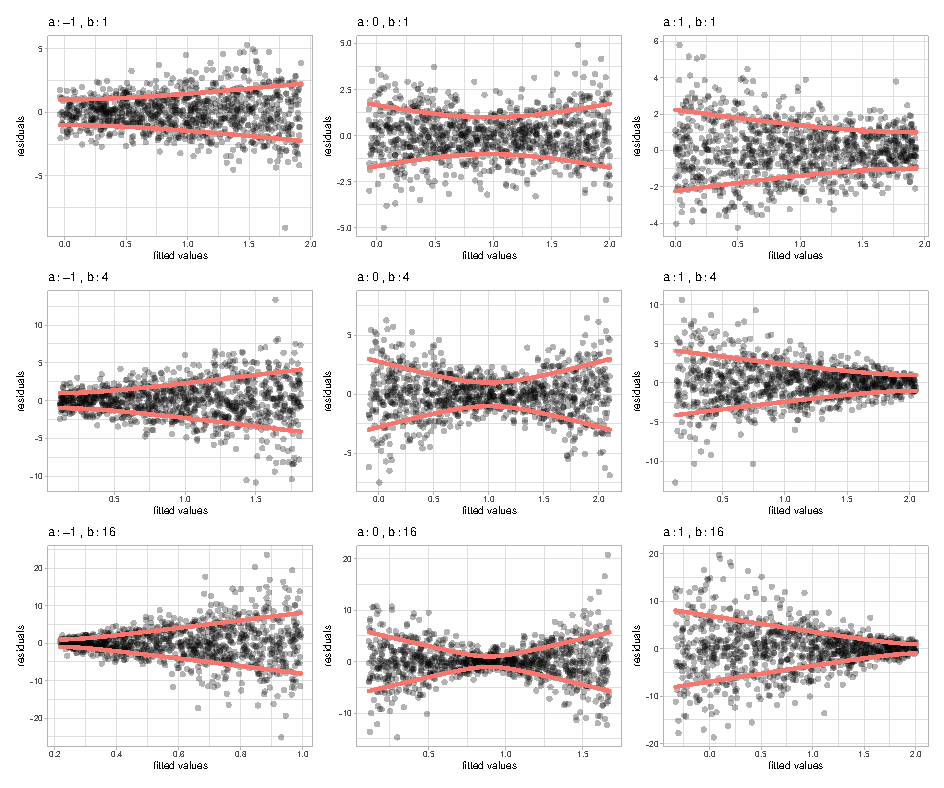
\includegraphics{thesis_files/figure-latex/hetershape-1.pdf}
\caption{\label{fig:hetershape}A matrix of residuals vs.~fitted values plot under different parameter settings of the heteroskedasticity model. Resdiauls are drawns in black and the one standard deviation around zero is drawn in red. The plots show that \(a\) controls the shape and direction of the resdiaul plot, while \(b\) controls the strength of the signal.}
\end{figure}

Similar to the cubic model, the heteroskedasticity model could also be built by the heteroskedasticity model class constructor \texttt{heter\_model()}. This function takes three arguments as inputs, which are \texttt{a}, \texttt{b} and \texttt{x}. \texttt{a} and \texttt{b} are numeric parameters defined in Equation (\ref{eq:heter}). \texttt{x} needs to be a random variable object.

\begin{Shaded}
\begin{Highlighting}[]
\FunctionTok{library}\NormalTok{(visage)}
\NormalTok{mod }\OtherTok{\textless{}{-}} \FunctionTok{heter\_model}\NormalTok{(}\AttributeTok{a =} \DecValTok{0}\NormalTok{, }\AttributeTok{b =} \DecValTok{16}\NormalTok{, }\AttributeTok{x =} \FunctionTok{rand\_uniform}\NormalTok{(}\SpecialCharTok{{-}}\DecValTok{1}\NormalTok{, }\DecValTok{1}\NormalTok{))}
\end{Highlighting}
\end{Shaded}

Since both the cubic model class and the heteroskedasticity class are inherited from the visual inference model class, which has defined methods of simulating data, making residual plot and producing lineup, heteroskedasticity model object can be used in a similar way as cubic model object. The following codes give examples of the use of the object.

\begin{Shaded}
\begin{Highlighting}[]
\NormalTok{mod}\SpecialCharTok{$}\FunctionTok{gen}\NormalTok{(}\DecValTok{5}\NormalTok{, }\AttributeTok{fit\_model =} \ConstantTok{TRUE}\NormalTok{)}
\end{Highlighting}
\end{Shaded}

\begin{verbatim}
##            y          x    sigma          e     .resid    .fitted
## 1 -7.6931740  0.8335218 4.819987 -9.5266958 -5.7469121 -1.9462619
## 2  7.0213194 -0.7458772 4.336202  6.7671966 -0.9130225  7.9343418
## 3 -2.1856528  0.9509873 5.471751 -4.1366401  0.4954643 -2.6811172
## 4  4.0402811  0.4961018 2.979219  2.5441792  3.8756685  0.1646126
## 5  0.8686919  0.7494172 4.355690 -0.8807253  2.2888017 -1.4201098
\end{verbatim}

\begin{Shaded}
\begin{Highlighting}[]
\NormalTok{mod}\SpecialCharTok{$}\FunctionTok{plot}\NormalTok{(mod}\SpecialCharTok{$}\FunctionTok{gen}\NormalTok{(}\DecValTok{100}\NormalTok{, }\AttributeTok{fit\_model =} \ConstantTok{TRUE}\NormalTok{), }\AttributeTok{size =} \DecValTok{1}\NormalTok{)}
\end{Highlighting}
\end{Shaded}

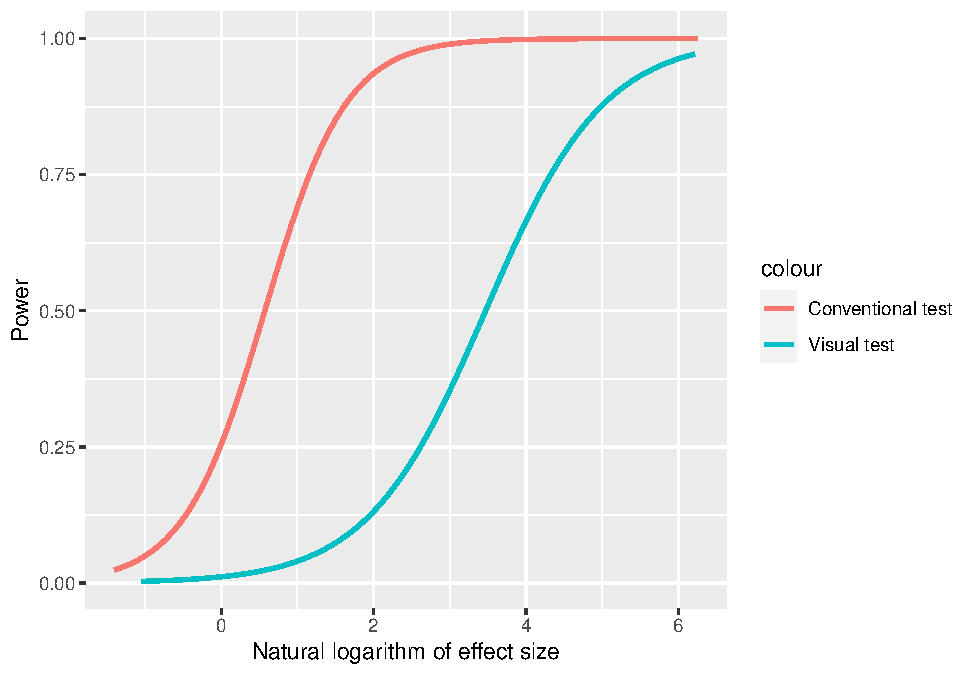
\includegraphics{thesis_files/figure-latex/unnamed-chunk-8-1.pdf}

\begin{Shaded}
\begin{Highlighting}[]
\NormalTok{mod}\SpecialCharTok{$}\FunctionTok{plot\_lineup}\NormalTok{(mod}\SpecialCharTok{$}\FunctionTok{gen\_lineup}\NormalTok{(}\DecValTok{100}\NormalTok{), }\AttributeTok{size =} \DecValTok{1}\NormalTok{)}
\end{Highlighting}
\end{Shaded}

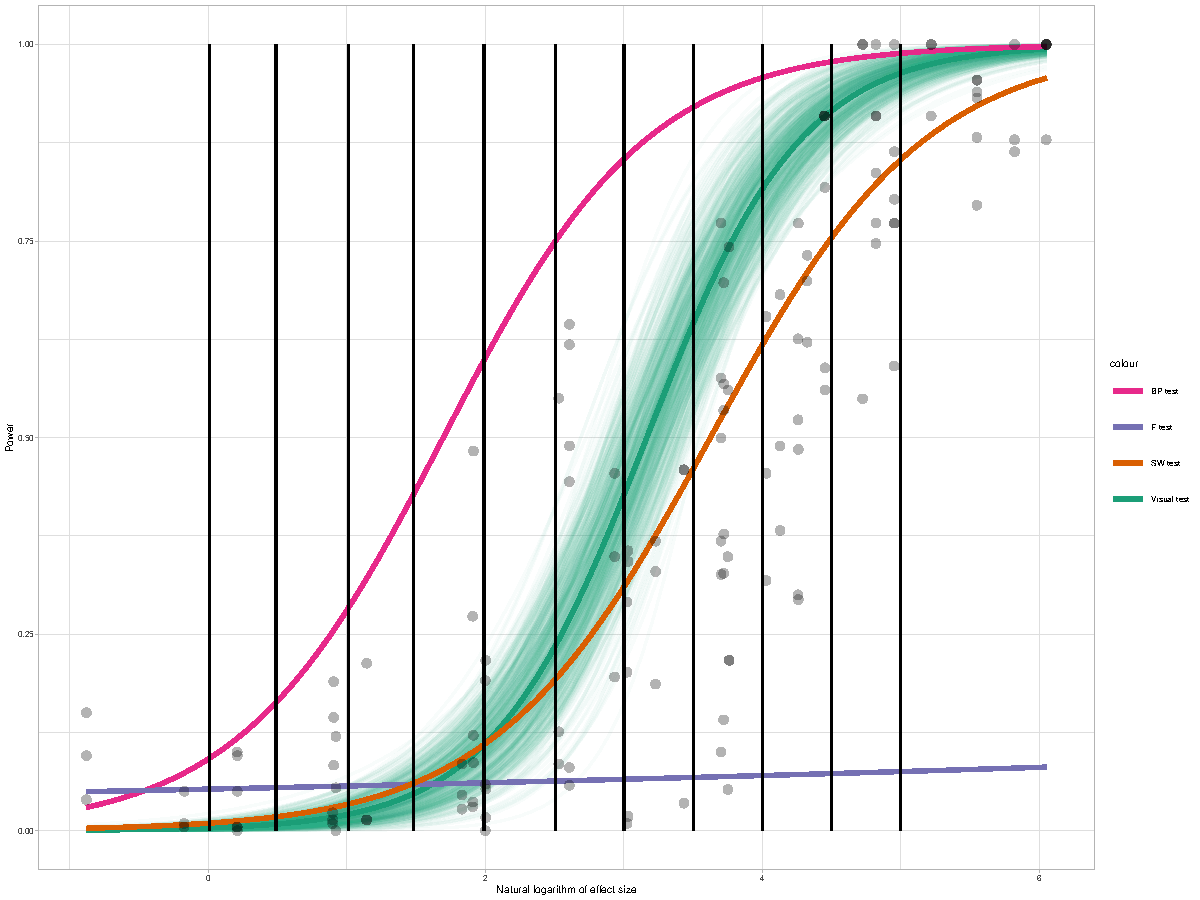
\includegraphics{thesis_files/figure-latex/unnamed-chunk-9-1.pdf}
According to Lemma \ref{lemma:heter}, when \(b = 0\), the matrix \(\boldsymbol{V}\) collapses to an identity matrix. Assume the shape of butterfly and triangle have identical visual impacts, the only factor affects human to recognize the pattern is the strength of the signal, where parameter \(a\) has no role to play. In addition, sample size has a huge impact on the chance of human recognizing the pattern. As shown in Figure \ref{fig:hetern}, as sample size increases, the pattern becomes easier to observe. However, this effect is less noticeable with large sample size as the outline of the shape has been drawn and residuals have less probability to land outside of it. Thus, the effect size of this model can be expressed by \(ES = b\sqrt{n}\). The square root operator is used for addressing the large sample issue. Figure \ref{fig:hetereffectsize} shows the effectiveness of the effect size.

\begin{figure}
\centering
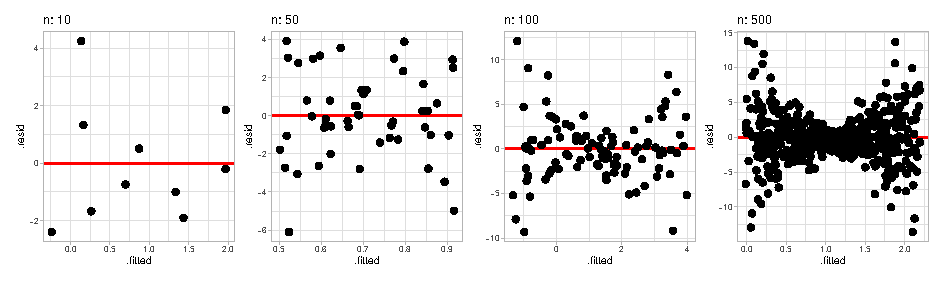
\includegraphics{thesis_files/figure-latex/hetern-1.pdf}
\caption{\label{fig:hetern}Residuals generated from the same heteroskedasticity model but with different sample size. As sample size increases, the shape of butterfly becomes more obvious.}
\end{figure}

\begin{figure}
\centering
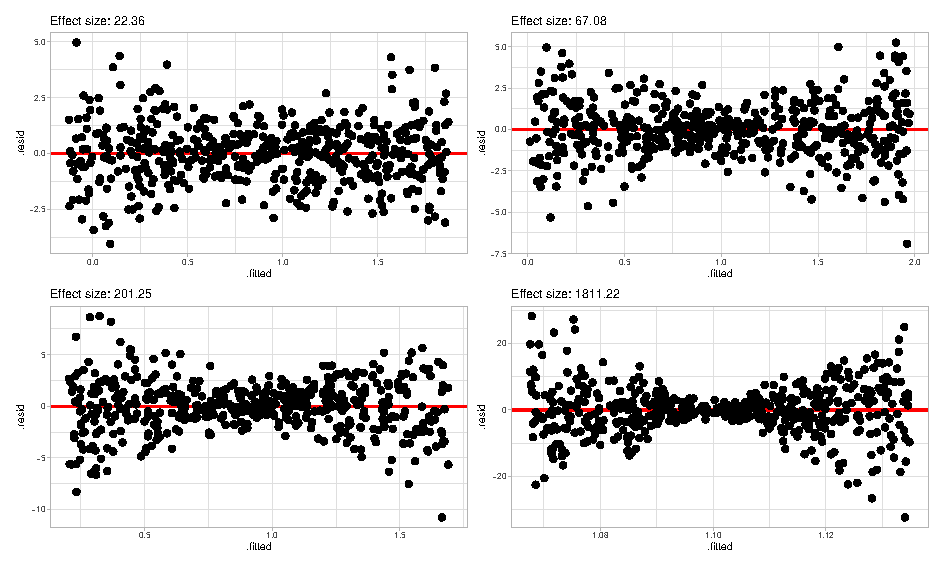
\includegraphics{thesis_files/figure-latex/hetereffectsize-1.pdf}
\caption{\label{fig:hetereffectsize}Residuals of heteroskedasticity model with different effect size. As effect size increases, the shape of butterfly becomes less noisy.}
\end{figure}

For the heteroskedasticity model, the conventional test we used was Breusch--Pagan test \autocite{breusch_simple_1979}, which tested whether the variance of the error terms of the regression is dependent on the regressors with the auxiliary regression equation \[\boldsymbol{e}^2 = \gamma_0 + \gamma_1 \boldsymbol{X} + \gamma_2 \boldsymbol{X}^2 + \boldsymbol{v}.\] \textcite{majumder_validation_2013} suggested that visual test is not expected to perform equally well as conventional test especially when there exists a exact conventional test. However, in contrast to the F-test used in the cubic model, Breusch--Pagan test is an approximate test. Thus, the power of visual test may exceed the power of Breusch--Pagan test. Throughout the study, Breusch--Pagan test statistic and p-value were recorded for comparison.

\hypertarget{distribution-of-regressors}{%
\subsection{Distribution of regressors}\label{distribution-of-regressors}}

The model definitions given in the previous two sections does not include the specification of the regressors. In this sections, distribution of \(\boldsymbol{X}\) and \(\boldsymbol{Z}\) will be discussed.

The cubic model involved the use of both \(\boldsymbol{X}\) and \(\boldsymbol{Z}\). In the simulation, \(X_i\), \(i=1,...,n\), had equal chance to follow one of the following distributions: \(N(0, 0.09)\), \(U(-1, 1)\), \(Lognormal(0,0.36)/3 - 1\) and \(-Lognormal(0,0.36)/3 + 1\). Uniform and normal distribution were symmetric and common. Adjusted lognormal distribution and adjusted negative lognormal distribution provided right-skewed and left-skewed density respectively. These distributions were chosen such that most the realizations will fall between \(-1\) and \(1\).

The distribution of \(Z_i\), \(i=1,...,n\), had \(50\)\% chance to be a uniform distribution ranged from \(-1\) to \(1\), and \(50\)\% chance to be a discrete uniform distribution with \(z_n\) outcomes simulated from a uniform distribution ranged from \(-1\) to \(1\). \(z_n\) itself was a discrete uniform distribution with outcomes \(\{10,11,12,13,14,15,16,17,18,19,20\}\), which defined the number of possible values \(Z_i\) could take. As shown in Figure \ref{fig:discreteex}, this setup would create discreteness in residual plot, which could enrich the pool of visual patterns.

\begin{figure}
\centering
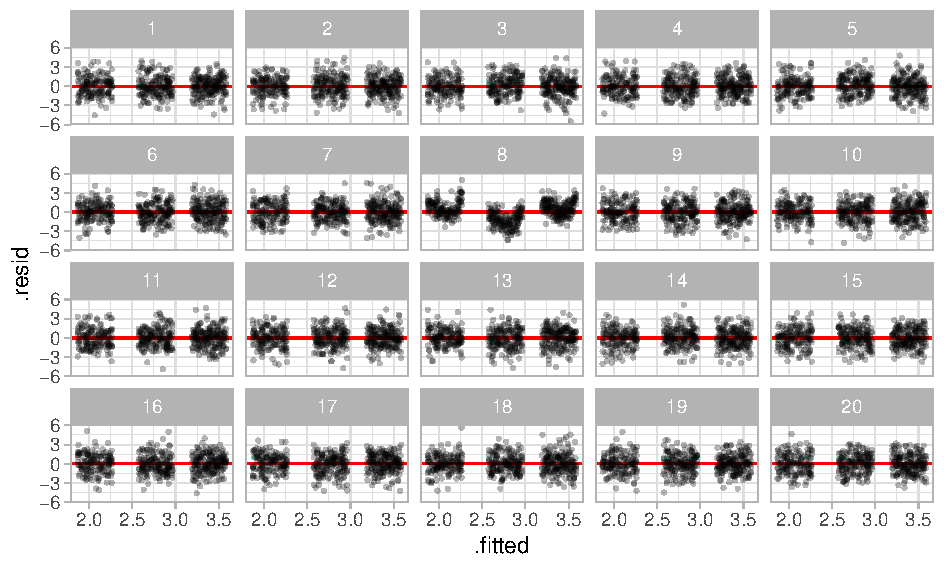
\includegraphics{thesis_files/figure-latex/discreteex-1.pdf}
\caption{\label{fig:discreteex}Discreteness in residuals created by using a discrete uniform random variable as one of the regressors in a cubic model. For each residual plot of the lineup, there are three clusters because the number of possible values the regressor can take is three.}
\end{figure}

\(\boldsymbol{X}\) used in the heteroskedasticity model was a combination of \(\boldsymbol{X}\) and \(\boldsymbol{Z}\) used in the cubic model. It could be one of the five distributions mentioned above - normal distribution, uniform distribution, adjusted lognormal distribution, adjusted negative lognormal distribution and discrete uniform distribution.

\hypertarget{experiment-i-and-ii}{%
\subsection{Experiment I and II}\label{experiment-i-and-ii}}

In this study, multiple selection was allowed for the evaluation of a lineup. Given our desired significance level was \(\alpha = 0.05\) and the number of plots in a lineup was \(20\), a single visual test procedure needed to involve multiple evaluations. Otherwise, the \(p\)-value of the test would be greater than \(0.05\) in spite of the actual data plot being selected. The number of plots selected by a user depended on the user and the difficulty of the lineup. According to the pilot study evaluated by \(10\) faculty members of Department of Econometrics and Business Analytics, Monash University, the number of selections would be generally smaller than \(4\), which suggested a visual test consisted of \(5\) evaluations were sufficient to yield \(p\)-value smaller than \(0.05\) with at least three detections. Thus, each lineup was replicated for five times and evaluated by different participants. However, our study website was designed such that any set of lineups consisting of 20 lineups generated beforehand would be shown to only one person only once. And whether the participant would finish the experiment was unpredictable. Therefore, some lineups had insufficient number of evaluations, but some had more evaluations than expected. This slightly affected the estimate of the power of the visual test, which will be discussed in Section \ref{p-value-and-power-estimation-of-visual-test-allowed-for-multiple-selections}.

We called the lineup being detected if the actual data plot was one of the selections of an evaluation of a lineup. The sample size calculation was based on the detection rate of the lineup, which was closely related to the difficulty level of the lineup. With the data collected from the pilot study, two logistic regressions given in Table \ref{tab:pilotglm} and Figure \ref{fig:pilotglm} were developed to describe the relationship between the natural logarithm of effect size and the detection rate for the cubic model and the heteroskedasticity model.

\begin{table}[!htbp] \centering 
  \caption{Logistic regressions with detection rate as response variable and natural logarithm of the effect size as regressor fitted on the pilot data for both cubic and heteroskedasticity models.} 
  \label{tab:pilotglm} 
\begin{tabular}{@{\extracolsep{5pt}}lcc} 
\\[-1.8ex]\hline 
\hline \\[-1.8ex] 
 & \multicolumn{2}{c}{\textit{Dependent variable:}} \\ 
\cline{2-3} 
\\[-1.8ex] & \multicolumn{2}{c}{detect} \\ 
 & Cubic & Heteroskedasticity \\ 
\\[-1.8ex] & (1) & (2)\\ 
\hline \\[-1.8ex] 
 log(effect\_size) & 0.611$^{***}$ & 0.737$^{***}$ \\ 
  & (0.098) & (0.137) \\ 
  & & \\ 
 Constant & 0.457$^{***}$ & $-$2.402$^{***}$ \\ 
  & (0.165) & (0.645) \\ 
  & & \\ 
\hline \\[-1.8ex] 
Observations & 246 & 289 \\ 
Log Likelihood & $-$122.305 & $-$147.971 \\ 
Akaike Inf. Crit. & 248.610 & 299.943 \\ 
\hline 
\hline \\[-1.8ex] 
\textit{Note:}  & \multicolumn{2}{r}{$^{*}$p$<$0.1; $^{**}$p$<$0.05; $^{***}$p$<$0.01} \\ 
\end{tabular} 
\end{table}

\begin{figure}
\centering
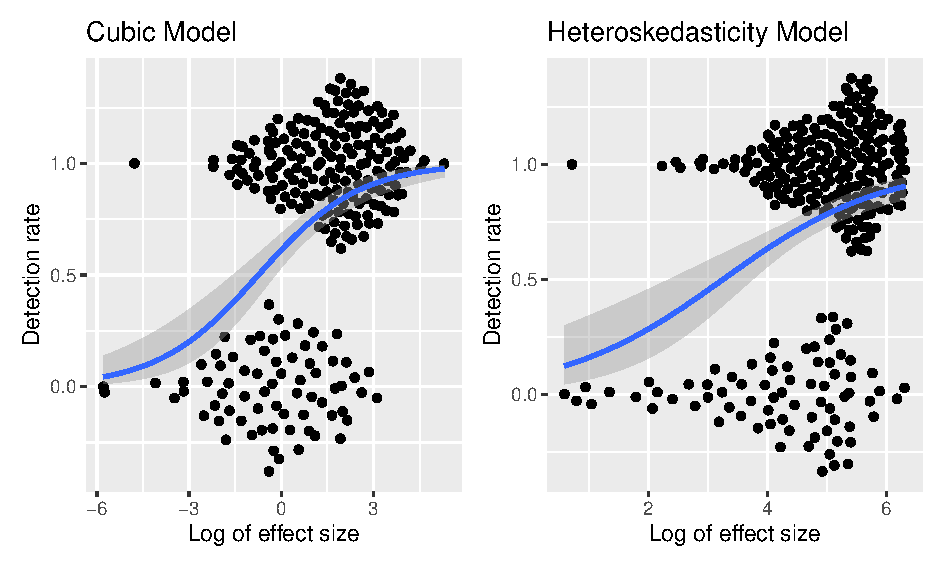
\includegraphics{thesis_files/figure-latex/pilotglm-1.pdf}
\caption{\label{fig:pilotglm}Logistic regressions with detection rate as response variable and natural logarithm of the effect size as regressor fitted on the pilot data for both cubic and heteroskedasticity models. Points are jittered to reduce overplotting using the \texttt{ggbeeswarm} package. The smooth curves are the fitted regression curves. The ribbons around the curves are the 95\% confidence intervals.}
\end{figure}

Lineups were classified into three categories - easy, medium and hard. Easy lineups were those of which predicted detection rates were higher than \(80\)\%, while medium lineups were between \(40\)\% to \(80\)\% and hard lineups were less than \(40\)\%.

For the first experiment, we would like to have at least 20 detection with chance greater than 99.99\% in each category. Thus, we prepared \(68\) easy lineups, \(120\) medium lineups and \(388\) hard lineups with five replications. Every participant would get at least \(8\) easy or medium lineups. Two out of \(10\) extremely lineups with predicted detection rate over \(90\)\% were randomly given to every participant as attention checks. We initially planned to recruit \((68+120+388) \times 5 / (20-2) = 160\) participants but eventually decided to only recruit \(20\) participants because it was the first time we launched an experiment on Prolific where factors like payment method and quality of participants were unclear at the moment. As a consequence, most of the lineups had only two evaluations and not all the lineups were used. However, data collected from the first experiment was sufficient for building a more accurate logistic regression to predict detection rate for the second experiment.

\begin{figure}
\centering
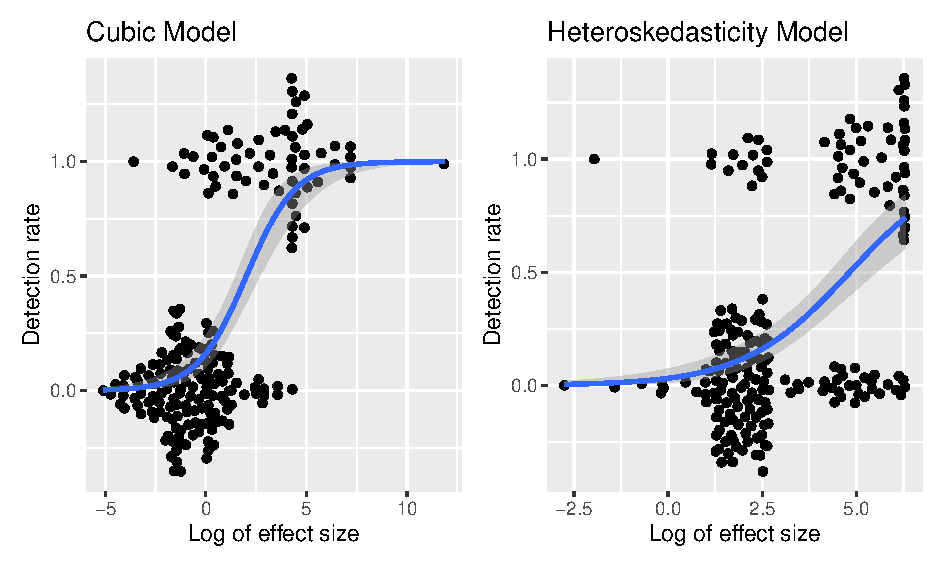
\includegraphics{thesis_files/figure-latex/e1glmplot-1.pdf}
\caption{\label{fig:e1glmplot}Logistic regressions with detection rate as response variable and natural logarithm of the effect size as regressor fitted on the data collected from experiment I for both cubic and heteroskedasticity models. Points are jittered to reduce overplotting using the \texttt{ggbeeswarm} package. The smooth curves are the fitted regression curves. The ribbons around the curves are the 95\% confidence intervals.}
\end{figure}

\begin{table}[!htbp] \centering 
  \caption{Logistic regressions with detection rate as response variable and natural logarithm of the effect size as regressor fitted on the data collected from experiment I for both cubic and heteroskedasticity models.} 
  \label{tab:e1glm} 
\begin{tabular}{@{\extracolsep{5pt}}lcc} 
\\[-1.8ex]\hline 
\hline \\[-1.8ex] 
 & \multicolumn{2}{c}{\textit{Dependent variable:}} \\ 
\cline{2-3} 
\\[-1.8ex] & \multicolumn{2}{c}{detect} \\ 
 & Cubic & Heteroskedasticity \\ 
\\[-1.8ex] & (1) & (2)\\ 
\hline \\[-1.8ex] 
 log(effect\_size) & 0.857$^{***}$ & 0.746$^{***}$ \\ 
  & (0.122) & (0.111) \\ 
  & & \\ 
 Constant & $-$1.571$^{***}$ & $-$3.434$^{***}$ \\ 
  & (0.257) & (0.462) \\ 
  & & \\ 
\hline \\[-1.8ex] 
Observations & 192 & 188 \\ 
Log Likelihood & $-$64.544 & $-$84.606 \\ 
Akaike Inf. Crit. & 133.089 & 173.212 \\ 
\hline 
\hline \\[-1.8ex] 
\textit{Note:}  & \multicolumn{2}{r}{$^{*}$p$<$0.1; $^{**}$p$<$0.05; $^{***}$p$<$0.01} \\ 
\end{tabular} 
\end{table}

According to the new logistic regression given in Table \ref{tab:e1glm} and Figure \ref{fig:e1glmplot}, it was found that the first experiment might be too difficult for participants as the detection rate was lower than what we estimated from the pilot study, especially for the heteroskedasticity model. Thus, for the second experiments, we relaxed the sample size requirements and increased the proportion of easy lineups. In addition, due to budget constraint, the maximum number of participants was \(50\). With the new logistic regression fitted with data collected from the first experiment, \(28\) easy lineups, \(36\) medium lineups and \(100\) hard lineups were simulated for the second experiment. \(50\) participants were recruited but \(6\) were withdrew.

\hypertarget{p-value-and-power-estimation-of-visual-test-allowed-for-multiple-selections}{%
\subsection{\texorpdfstring{\(P\)-value and Power Estimation of Visual Test Allowed for Multiple Selections}{P-value and Power Estimation of Visual Test Allowed for Multiple Selections}}\label{p-value-and-power-estimation-of-visual-test-allowed-for-multiple-selections}}

The \(p\)-value calculation for multiple selection is an extension of Equation (\ref{eq:pvaluesingle}). The assumptions about the independence still needed. Let \(K\) be the number of independent evaluations of a visual test, \(s_i\), \(i = 1,...,K\) be the number of selections of the evaluations, and \(X\) be the random variable denoting the number of detections. Then, the \(p\)-value of the visual test is given as:
\begin{equation} \label{eq:pvaluemulti}
P(X\geq x) = \sum_{j=x}^{K}Pr(j|s_1,...,s_K).
\end{equation}
The distribution of \(X\) given \(s_1,...s_K\) can not be derived trivially, as it is a sampling without replacement problem. In practice, this distribution can be approximated by computer simulation.

Function \texttt{sim\_dist()} from package \texttt{visage} is designed to approximate the distribution of number of detections of a lineup via Monte Carlo method. It takes the number of evaluations \texttt{n\_eval}, the number of selections \texttt{n\_sel}, and the number of plots in a lineup \texttt{n\_plot} as inputs, then outputs a discrete distribution.

\begin{Shaded}
\begin{Highlighting}[]
\FunctionTok{sim\_dist}\NormalTok{(}\AttributeTok{n\_eval =} \DecValTok{3}\NormalTok{, }\AttributeTok{n\_sel =} \FunctionTok{c}\NormalTok{(}\DecValTok{2}\NormalTok{, }\DecValTok{2}\NormalTok{, }\DecValTok{3}\NormalTok{), }\AttributeTok{n\_plot =} \DecValTok{20}\NormalTok{)}
\end{Highlighting}
\end{Shaded}

\begin{verbatim}
##       0       1       2       3 
## 0.70094 0.25280 0.04340 0.00286
\end{verbatim}

Function \texttt{calc\_p\_value()} from the same package calculates the \(p\)-value using the distribution returned by \texttt{sim\_dist()}. It takes an additional argument \texttt{n\_detect}, which is the number of detections.

\begin{Shaded}
\begin{Highlighting}[]
\FunctionTok{calc\_p\_value}\NormalTok{(}\AttributeTok{n\_detect =} \DecValTok{2}\NormalTok{, }\AttributeTok{n\_eval =} \DecValTok{3}\NormalTok{, }\AttributeTok{n\_sel =} \FunctionTok{c}\NormalTok{(}\DecValTok{2}\NormalTok{, }\DecValTok{2}\NormalTok{, }\DecValTok{3}\NormalTok{), }\AttributeTok{n\_plot =} \DecValTok{20}\NormalTok{)}
\end{Highlighting}
\end{Shaded}

\begin{verbatim}
## [1] 0.0456
\end{verbatim}

The above example shows that a visual test with two detections and three independent evaluations in which three observers select two, two, and three plots out of \(20\) plots respectively yields a \(p\)-value smaller than \(0.05\).

Assume there is a visual test \(V_K\), where \(K\) denoting the number of evaluations. The corresponding \(p\)-value of \(V_K\) can be computed by using Equation (\ref{eq:pvaluemulti}). Meanwhile, if one evaluation is randomly deleted from \(V_K\), the remaining evaluations can still be used to form another valid visual test \(V_{K-1}\). In fact, considering all the possibilities, \(K\) different outcomes for \(V_{K-1}\) can be obtained. Since all outcomes occur with equal probability, the proportion of outcomes which reject the null hypothesis can be used as an estimate of the power of the visual test \(V_{K-1}\). Similarly, if we would like to estimate the power of the visual test \(V_{K-j}\) given the evaluations of \(V_{K}\), for \(j < K\), we could find all the possible combinations of \(K\) elements, taken \(k-j\) at a time to obtain \(K\choose{K-j}\) different outcomes for \(V_{K-j}\). Then, the estimated power is given as \(R/{K\choose{K-j}}\), where \(R\) is the number of outcomes which reject the null hypothesis.

Function \texttt{calc\_p\_value\_comb()} from the package \texttt{visage} can be used to compute \(p\)-values of \(V_{K-j}\). The first argument is \texttt{detected}, which needs to be a vector of Boolean values denoting whether the observer detects the actual data plot. Desired number of evaluations and number of selections need to be provided via argument \texttt{n\_eval} and \texttt{n\_sel}.

For example, given a visual test \(V_3\) where the first observer selects one plot and gets correct, the second observer selects one plot but misses, and the third observer selects two plots and gets correct. The \(p\)-value of all possible outcomes of \(V_2\) can be computed using the following code:

\begin{Shaded}
\begin{Highlighting}[]
\FunctionTok{calc\_p\_value\_comb}\NormalTok{(}\AttributeTok{detected =} \FunctionTok{c}\NormalTok{(}\ConstantTok{TRUE}\NormalTok{, }\ConstantTok{FALSE}\NormalTok{, }\ConstantTok{TRUE}\NormalTok{), }
                  \AttributeTok{n\_eval =} \DecValTok{2}\NormalTok{, }
                  \AttributeTok{n\_sel =} \FunctionTok{c}\NormalTok{(}\DecValTok{1}\NormalTok{, }\DecValTok{1}\NormalTok{, }\DecValTok{2}\NormalTok{))}
\end{Highlighting}
\end{Shaded}

\begin{verbatim}
## [1] 0.09352 0.00624 0.14454
## attr(,"combinations")
##      [,1] [,2] [,3]
## [1,]    1    1    2
## [2,]    2    3    3
\end{verbatim}

\texttt{calc\_p\_value\_comb()} returns a vector of \(p\)-value along with an attribute which is a matrix representing elements being used by the specific outcome. Elements in the first column indicates that the first observer and the second observer are involved in the visual test, and the corresponding \(p\)-value is \(0.09352\).

\hypertarget{results}{%
\subsection{Results}\label{results}}

We collected \(400\) lineup evaluations made by \(20\) participants in experiment I and \(880\) lineup evaluations made by \(44\) participants in experiment II. In total, \(442\) unique lineups were evaluated by \(64\) subjects. In experiment I, one of the participants skipped all \(20\) lineups. Hence, the submission was rejected and removed from the dataset. In experiment II, there was a participant failed one of the two attention checks, but there was no further evidence of low-effort throughout the experiment. Therefore, the submission was kept.

\hypertarget{power-estimation}{%
\subsubsection{Power Estimation}\label{power-estimation}}

It was expected that with larger effect size, the power of the visual test would be greater for both cubic model and heteroskedasticity model. Using the power calculation method discussed in Section \ref{p-value-and-power-estimation-of-visual-test-allowed-for-multiple-selections}, power of each lineup from one to five evaluations was estimated. The estimated power was further used in fitting a quasi-binomial generalized linear model with natural logarithm of effect size as the only regressor. The result of the fitted models are given in Table \ref{tab:powerglmcubic}, Table \ref{tab:powerglmheter}, and Figure \ref{fig:powerglm}.

As expected, coefficients of natural logarithm of effect size of all five models were positive. From Figure \ref{fig:powerglm}, it can be observed that the fitted power of visual test increased as the number of evaluations increased for both cubic and heteroskedasticity model.

For heteroskedasticity model, this phenomenon was more obvious as the curves of visual tests with evaluations greater than two were always above the curves of visual test with evaluations smaller than two. However, this only held for large enough effect size. For small effect size, visual tests with fewer evaluations might have greater power. Note that, the expected power of visual test derived by \textcite{majumder_validation_2013} followed by the assumption that human has the ability to select the plot with the highest t-statistic from a lineup under the classical linear model regression setting showed similar properties, where visual tests with fewer evaluations were expected to perform better when the parameter values close to the null hypothesis.

For cubic model, the separation between curves was small. Fitted power of visual test with three to five evaluations were almost identical to each other in regards of effect size. In addition, all five curves peaked at one as effect size increased, suggesting that identification of nonlinearity as a visual task can be completed reliably by human when the effect size is large enough.

As shown in Figure \ref{fig:powerglm}, both F-test and Breusch--Pagan test generally possessed greater power than visual test. Since the settings we were using were not ideal scenarios for visual inference, it was not expected that the visual test would be as good as the conventional test. Our goal was to quantify the ability of human reading residual plot, such that the comparison between human and computer vision model can be made.

\begin{table}[!htbp] \centering 
  \caption{Quasi-binomial logistic regressions with estimated power as response variable and natural logarithm of the effect size as regressor fitted on the data collected from experiment I and II for cubic model. Five regressions were fitted for different number of evaluations.} 
  \label{tab:powerglmcubic} 
\begin{tabular}{@{\extracolsep{5pt}}lccccc} 
\\[-1.8ex]\hline 
\hline \\[-1.8ex] 
 & \multicolumn{5}{c}{\textit{Dependent variable:}} \\ 
\cline{2-6} 
\\[-1.8ex] & \multicolumn{5}{c}{hat\_power} \\ 
\\[-1.8ex] & (1) & (2) & (3) & (4) & (5)\\ 
\hline \\[-1.8ex] 
 log(effect\_size) & 0.929$^{***}$ & 1.227$^{***}$ & 1.084$^{***}$ & 1.057$^{***}$ & 1.035$^{***}$ \\ 
  & (0.049) & (0.066) & (0.074) & (0.082) & (0.087) \\ 
  & & & & & \\ 
 Constant & $-$1.969$^{***}$ & $-$2.603$^{***}$ & $-$1.570$^{***}$ & $-$1.501$^{***}$ & $-$1.432$^{***}$ \\ 
  & (0.114) & (0.153) & (0.142) & (0.156) & (0.160) \\ 
  & & & & & \\ 
\hline \\[-1.8ex] 
Observations & 630 & 532 & 456 & 423 & 371 \\ 
\hline 
\hline \\[-1.8ex] 
\textit{Note:}  & \multicolumn{5}{r}{$^{*}$p$<$0.1; $^{**}$p$<$0.05; $^{***}$p$<$0.01} \\ 
\end{tabular} 
\end{table}

\begin{table}[!htbp] \centering 
  \caption{Quasi-binomial logistic regressions with estimated power as response variable and natural logarithm of the effect size as regressor fitted on the data collected from experiment I and II for heteroskedasticity model. Five regression were fitted for different number of evaluations.} 
  \label{tab:powerglmheter} 
\begin{tabular}{@{\extracolsep{5pt}}lccccc} 
\\[-1.8ex]\hline 
\hline \\[-1.8ex] 
 & \multicolumn{5}{c}{\textit{Dependent variable:}} \\ 
\cline{2-6} 
\\[-1.8ex] & \multicolumn{5}{c}{hat\_power} \\ 
\\[-1.8ex] & (1) & (2) & (3) & (4) & (5)\\ 
\hline \\[-1.8ex] 
 log(effect\_size) & 0.821$^{***}$ & 1.025$^{***}$ & 0.885$^{***}$ & 0.920$^{***}$ & 1.063$^{***}$ \\ 
  & (0.064) & (0.087) & (0.092) & (0.102) & (0.125) \\ 
  & & & & & \\ 
 Constant & $-$4.472$^{***}$ & $-$5.610$^{***}$ & $-$4.285$^{***}$ & $-$4.127$^{***}$ & $-$4.717$^{***}$ \\ 
  & (0.320) & (0.449) & (0.461) & (0.499) & (0.607) \\ 
  & & & & & \\ 
\hline \\[-1.8ex] 
Observations & 630 & 527 & 473 & 443 & 375 \\ 
\hline 
\hline \\[-1.8ex] 
\textit{Note:}  & \multicolumn{5}{r}{$^{*}$p$<$0.1; $^{**}$p$<$0.05; $^{***}$p$<$0.01} \\ 
\end{tabular} 
\end{table}

\begin{figure}
\centering
\includegraphics{thesis_files/figure-latex/powerglm-1.pdf}
\caption{\label{fig:powerglm}Quasi-binomial logistic regressions with estimated power as response variable and natural logarithm of the effect size as regressor fitted on the data collected from experiment I and II for both cubic and heteroskedasticity model. Five regression were fitted for different number of evaluations shown in five different colours. Estimated power are drawn in black. The dashed curvses are the power of F-test and Breusch--Pagan test respectively.}
\end{figure}

Another method we used to model the power was to collect all decisions made by \(K\choose{K-j}\) different outcomes for \(V_{K-j}\), and directly fit a binomial generalized linear model with natural logarithm of effect size as the regressor. This method skipped the calculation of the estimated power \(R/{K\choose{K-j}}\), and regressed on the binary outcome with larger sample size. Results of the fitted model is given in Figure \ref{fig:powerglmsecond}, Table \ref{tab:powerglmhetersecond} and Table \ref{tab:powerglmcubicsecond}. According to Figure \ref{fig:powerglmsecond}, this method gave clearer separation between curves for heteroskedasticity model. Noticeably, fitted power of visual test with five evaluations matched the power of conventional test at large effect size.

\begin{table}[!htbp] \centering 
  \caption{Logistic regressions with rejection as response variable and natural logarithm of the effect size as regressor fitted on the data collected from experiment I and II for cubic model. Five regression were fitted for different number of evaluations.} 
  \label{tab:powerglmcubicsecond} 
\begin{tabular}{@{\extracolsep{5pt}}lccccc} 
\\[-1.8ex]\hline 
\hline \\[-1.8ex] 
 & \multicolumn{5}{c}{\textit{Dependent variable:}} \\ 
\cline{2-6} 
\\[-1.8ex] & \multicolumn{5}{c}{hat\_power} \\ 
\\[-1.8ex] & (1) & (2) & (3) & (4) & (5)\\ 
\hline \\[-1.8ex] 
 log(effect\_size) & 0.872$^{***}$ & 1.292$^{***}$ & 1.125$^{***}$ & 1.164$^{***}$ & 1.315$^{***}$ \\ 
  & (0.031) & (0.032) & (0.021) & (0.021) & (0.029) \\ 
  & & & & & \\ 
 Constant & $-$1.836$^{***}$ & $-$2.529$^{***}$ & $-$1.516$^{***}$ & $-$1.321$^{***}$ & $-$1.419$^{***}$ \\ 
  & (0.077) & (0.073) & (0.046) & (0.049) & (0.072) \\ 
  & & & & & \\ 
\hline \\[-1.8ex] 
Observations & 2,900 & 7,250 & 12,596 & 17,011 & 19,229 \\ 
Log Likelihood & $-$752.896 & $-$1,312.436 & $-$2,977.445 & $-$2,651.299 & $-$1,463.555 \\ 
Akaike Inf. Crit. & 1,509.792 & 2,628.873 & 5,958.889 & 5,306.598 & 2,931.109 \\ 
\hline 
\hline \\[-1.8ex] 
\textit{Note:}  & \multicolumn{5}{r}{$^{*}$p$<$0.1; $^{**}$p$<$0.05; $^{***}$p$<$0.01} \\ 
\end{tabular} 
\end{table}

\begin{table}[!htbp] \centering 
  \caption{Logistic regressions with rejection as response variable and natural logarithm of the effect size as regressor fitted on the data collected from experiment I and II for heteroskedasticity model. Five regression were fitted for different number of evaluations.} 
  \label{tab:powerglmhetersecond} 
\begin{tabular}{@{\extracolsep{5pt}}lccccc} 
\\[-1.8ex]\hline 
\hline \\[-1.8ex] 
 & \multicolumn{5}{c}{\textit{Dependent variable:}} \\ 
\cline{2-6} 
\\[-1.8ex] & \multicolumn{5}{c}{hat\_power} \\ 
\\[-1.8ex] & (1) & (2) & (3) & (4) & (5)\\ 
\hline \\[-1.8ex] 
 log(effect\_size) & 0.912$^{***}$ & 1.221$^{***}$ & 1.294$^{***}$ & 1.525$^{***}$ & 1.798$^{***}$ \\ 
  & (0.044) & (0.033) & (0.027) & (0.030) & (0.042) \\ 
  & & & & & \\ 
 Constant & $-$4.846$^{***}$ & $-$6.396$^{***}$ & $-$6.033$^{***}$ & $-$6.771$^{***}$ & $-$7.784$^{***}$ \\ 
  & (0.229) & (0.175) & (0.141) & (0.159) & (0.230) \\ 
  & & & & & \\ 
\hline \\[-1.8ex] 
Observations & 2,906 & 7,064 & 11,436 & 13,728 & 13,236 \\ 
Log Likelihood & $-$1,525.398 & $-$3,668.325 & $-$5,491.915 & $-$4,828.896 & $-$2,858.774 \\ 
Akaike Inf. Crit. & 3,054.796 & 7,340.650 & 10,987.830 & 9,661.793 & 5,721.548 \\ 
\hline 
\hline \\[-1.8ex] 
\textit{Note:}  & \multicolumn{5}{r}{$^{*}$p$<$0.1; $^{**}$p$<$0.05; $^{***}$p$<$0.01} \\ 
\end{tabular} 
\end{table}

\begin{figure}
\centering
\includegraphics{thesis_files/figure-latex/powerglmsecond-1.pdf}
\caption{\label{fig:powerglmsecond}Logistic regressions with rejection as response variable and natural logarithm of the effect size as regressor fitted on the data collected from experiment I and II for both cubic and heteroskedasticity model. Five regression were fitted for different number of evaluations shown in five different colours. Estimated power are drawn in black. The dashed curvses are the power of F-test and Breusch--Pagan test respectively.}
\end{figure}

\hypertarget{effect-of-factors-on-power-of-the-visual-test}{%
\subsubsection{Effect of Factors on Power of the Visual Test}\label{effect-of-factors-on-power-of-the-visual-test}}

The previous section focuses on the change of effect size relative to the power of the visual test. Individual factor embedded in the data simulation also needs be analysed. Two logistic regressions were fitted with decisions made by \(V_{K-j}\) as response variable. For the cubic model, regressors were \(|a|\), \(|b|\), \(|c-1|\), \(\sigma\), distribution of \(\boldsymbol{X}\), distribution of \(\boldsymbol{Z}\), number of observations and number of evaluations. For the heteroskedasticity model, regressors were \(|a|\), \(b\), distribution of \(\boldsymbol{X}\), number of observations and number of evaluations.

According to Table \ref{tab:rejectfactorcubic}, for cubic model, both coefficients of \(|a|\) and \(|b|\) were positive, which suggested increasing the coefficients of quadric and cubic terms would result in higher visual power. The coefficient of \(|c-1|\) was also positive indicating joint effect of multiple regressors on the residual plot decreased the visual power. As expected, the coefficient of \(\sigma\) was negative as it controlled the noise level. Lineup simulated with uniform distribution of \(\boldsymbol{X}\) had the highest power, followed by negative lognormal, normal, and lognormal. Discreteness in \(\boldsymbol{Z}\) decreased the visual power. The coefficient of number of observations was positive, which means larger sample size would lead to higher visual power.

Results of logistic regression for heteroskedasticity is given in Table \ref{tab:rejectfactorheter}. For heteroskedasticity model, the coefficient of \(|a|\) was negative, which suggested ``butter fly'' shape was easier to identify than ``triangle'' shape. As expected, the coefficient of \(b\) was positive. For different distributions of \(\boldsymbol{X}\), the one with highest power was uniform distribution, followed by normal, discrete uniform, lognormal and negative lognormal. The coeffient of the number of observations was positive, but it was not significant.

In overall, we did not have any unexpected findings except the visual power related to different distributions of \(\boldsymbol{X}\) in cubic model. We expected lineup simulated with uniform distribution would have the highest power, followed by normal, lognormal and negative lognormal, since we observed similar results in pilot study.

\begin{table}[!htbp] \centering 
  \caption{Logistic regressions with rejection as response variable and parameter settings as regressors fitted on the data collected from experiment I and II for cubic model.} 
  \label{tab:rejectfactorcubic} 
\begin{tabular}{@{\extracolsep{5pt}}lc} 
\\[-1.8ex]\hline 
\hline \\[-1.8ex] 
 & \multicolumn{1}{c}{\textit{Dependent variable:}} \\ 
\cline{2-2} 
\\[-1.8ex] & reject \\ 
\hline \\[-1.8ex] 
 |a| & 1.064$^{***}$ \\ 
  & (0.031) \\ 
  & \\ 
 |b| & 0.718$^{***}$ \\ 
  & (0.029) \\ 
  & \\ 
 |c-1| & 5.443$^{***}$ \\ 
  & (0.119) \\ 
  & \\ 
 sigma & $-$3.536$^{***}$ \\ 
  & (0.050) \\ 
  & \\ 
 Distribution of X: Negative Lognormal & 0.971$^{***}$ \\ 
  & (0.073) \\ 
  & \\ 
 Distribution of X: Normal & 0.754$^{***}$ \\ 
  & (0.086) \\ 
  & \\ 
 Distribution of X: Uniform & 1.751$^{***}$ \\ 
  & (0.085) \\ 
  & \\ 
 Distribution of Z: Discrete & $-$2.986$^{***}$ \\ 
  & (0.056) \\ 
  & \\ 
 n & 0.005$^{***}$ \\ 
  & (0.0002) \\ 
  & \\ 
 Number of evaluations & 0.291$^{***}$ \\ 
  & (0.017) \\ 
  & \\ 
 Constant & $-$2.453$^{***}$ \\ 
  & (0.173) \\ 
  & \\ 
\hline \\[-1.8ex] 
Observations & 58,986 \\ 
Log Likelihood & $-$8,034.351 \\ 
Akaike Inf. Crit. & 16,090.700 \\ 
\hline 
\hline \\[-1.8ex] 
\textit{Note:}  & \multicolumn{1}{r}{$^{*}$p$<$0.1; $^{**}$p$<$0.05; $^{***}$p$<$0.01} \\ 
\end{tabular} 
\end{table}

\begin{table}[!htbp] \centering 
  \caption{Logistic regressions with rejection as response variable and parameter settings as regressors fitted on the data collected from experiment I and II for heteroskedasticity model.} 
  \label{tab:rejectfactorheter} 
\begin{tabular}{@{\extracolsep{5pt}}lc} 
\\[-1.8ex]\hline 
\hline \\[-1.8ex] 
 & \multicolumn{1}{c}{\textit{Dependent variable:}} \\ 
\cline{2-2} 
\\[-1.8ex] & reject \\ 
\hline \\[-1.8ex] 
 |a| & $-$0.526$^{***}$ \\ 
  & (0.037) \\ 
  & \\ 
 b & 0.064$^{***}$ \\ 
  & (0.002) \\ 
  & \\ 
 Distribution of X: Lognormal & $-$0.534$^{***}$ \\ 
  & (0.058) \\ 
  & \\ 
 Distribution of X: Negative Lognormal & $-$0.610$^{***}$ \\ 
  & (0.062) \\ 
  & \\ 
 Distribution of X: Normal & 0.187$^{***}$ \\ 
  & (0.063) \\ 
  & \\ 
 Distribution of X: Uniform & 2.980$^{***}$ \\ 
  & (0.064) \\ 
  & \\ 
 n & 0.0003 \\ 
  & (0.0002) \\ 
  & \\ 
 Number of evaluations & 0.496$^{***}$ \\ 
  & (0.014) \\ 
  & \\ 
 Constant & $-$2.711$^{***}$ \\ 
  & (0.062) \\ 
  & \\ 
\hline \\[-1.8ex] 
Observations & 48,370 \\ 
Log Likelihood & $-$13,026.190 \\ 
Akaike Inf. Crit. & 26,070.390 \\ 
\hline 
\hline \\[-1.8ex] 
\textit{Note:}  & \multicolumn{1}{r}{$^{*}$p$<$0.1; $^{**}$p$<$0.05; $^{***}$p$<$0.01} \\ 
\end{tabular} 
\end{table}

\hypertarget{automatic-visual-inference-system}{%
\section{Automatic Visual Inference System}\label{automatic-visual-inference-system}}

Lineup protocol can be used to make valid inference for visual discoveries, but one of the drawbacks of this protocol is it requires human evaluation of data plots. Such requirement is unattainable when the number of data plots need for testing is large. Even if it can be fulfilled, the cost of labour would be exceedingly high. Hence, there is a need of building an automatic visual inference system to read data plots, evaluate lineups and provide meaningful decisions. Since this desired automatic system is technically an agent intended to play the role of evaluators as humans in lineup protocol, some degree of intelligence needs to be demonstrated. This brings us to Artificial Intelligence (AI).

\hypertarget{se:ai}{%
\subsection{Artificial Intelligence: Four Approaches}\label{se:ai}}

AI is the field of research concerned with understanding and building machines who can demonstrate intelligence. As discussed in \textcite{russell_artificial_2002}, historically, there are disagreements among researchers about the definition of intelligence, which is caused by two critical questions:

\begin{enumerate}
\def\labelenumi{\arabic{enumi}.}
\tightlist
\item
  Should AI act and think humanly or rationally?
\item
  Without the thought process and reasoning, are behaviours sufficient to demonstrate intelligence?
\end{enumerate}

Based on the answer to the above questions, four major approaches to pursue AI have been established. These approaches can be summarized into a two by two table as shown in Figure \ref{fig:two-dim-ai}, where the row is ``Human'' vs.~``Rational'', and the column is ``Behaviour'' vs.~``Thought''. Positioning at the top right cell, the rational agent approach aims to build agent that perform mathematically perfect acts such that the best expected outcome can always be achieved. In contrast, the ``laws of thought'' approach focus on understanding the logic behind the rationality. Closely related to cognitive science, the cognitive modelling approach attempts to express theories of human cognition as computer program to mimic the thought process of human. Lastly, the Turing test approach is built upon the famous Turing test proposed by \textcite{turing_computing_1950}. The test can be roughly described as, whether a human can distinguish another human from a computer with written communications only. To pass the test, several capabilities of computer are required. This includes natural language processing for communication with human, knowledge representation for encoding knowledge, automated reasoning for derivation of conclusions and machine learning for improving AI automatically through experience and data. Some researchers argued that written communication is insufficient to demonstrate intelligence, and some degree of physical simulation of a person is still necessary. One such example is the total Turing test proposed by \textcite{harnad_other_1991}. It adds three new requirements to the list, including computer vision, speech recognition and robotics, which are response for interactions with the physical world. Notably, all seven required capabilities have become major subfields of AI today. And their development has made AI one of the fastest-growing fields in the 21st century \autocite{russell_artificial_2002}.

\begin{figure}
\centering
\includegraphics{thesis_files/figure-latex/two-dim-ai-1.pdf}
\caption{\label{fig:two-dim-ai}Four possible approaches to pursue AI based on the two dimensions in AI research - human vs.~rational and thought vs.~behavior \autocite{russell_artificial_2002}.}
\end{figure}

Considering there are different approches of AI, it is necessary to clarify the type of AI we aimed to build. Understanding the human thought process or mimicking the human vision mechanism were not of interest in this research. We believed humanly behaviours was enough for demonstrating AI for the problem we concerned. Hence, two of the capacities required by the total Turing test, namely machine learning and computer vision were adopted.

Another possible method under the rational agent approach was to define distance metrics to measure difference between data plots for making mathematically prefect decisions. This method would work if such metrics can be obtained manually or approximated algorithmically. However, we considered it was too complex to fit into our prototype automatic system. But we will revisited this method in our second project.

\hypertarget{design-of-the-automatic-system}{%
\subsection{Design of the Automatic System}\label{design-of-the-automatic-system}}

Depended on the inputs and outputs of the automatic system, various designs arised.

A system can be summarised

For an automatic visual inference system, types of inputs can be classified by two decisions: (i) whether to accept multiple image files as inputs, and (ii) whether to accept fitted model.

single image file
multiple image files

fitted model

Depend on the inputs and outputs, computer vision model can be integrated into an automatic visual inference system.

\hypertarget{different-approaches-of-ai}{%
\subsection{different approaches of AI}\label{different-approaches-of-ai}}

\begin{itemize}
\tightlist
\item
  Not aim for understanding the thought process
\item
  Not aim for mimicking the human vision mechanism
\item
  May be able to define distance metrics to measure difference between data plots for making mathematically prefect decisions
\item
  May be able to use computer vision model to approximate how people evaluate lineups
\end{itemize}

computer vision model:

\begin{itemize}
\tightlist
\item
  Use human data to train model with human selection as target -\textgreater{} mimic the human behaviour
\item
  Use simulated lineup to train model with actual data plot as target -\textgreater{} assume the actual data plot is the most different one
\item
  Use simulated data plot to train model with null or not null as target -\textgreater{} limited to the alternatives given to the model, and Type I error can not be controlled
\item
  Use simulated data plot to train model, then let the model evaluate each plot of a lineup -\textgreater{} leads to multiple selections in a lineup, and the model does not compare different plots in a lineup

  \begin{itemize}
  \tightlist
  \item
    Use a very large \(m\) to ensure the null hypothesis can be rejected by a classifier slightly better than a random selector. The problem becomes how large the \(m\) should be
  \item
    Use multiple models as multiple individuals to evaluate lineup -\textgreater{} Which models should be used? How many models should be used?
  \end{itemize}
\item
  Let the model select multiple plots from a simulated lineup while comparing different plots in a lineup -\textgreater{} how to build such a system?

  \begin{itemize}
  \tightlist
  \item
    The input is \(m\) plots, what is the output? The probability of being the most different one?
  \item
    Then how many plots should be selected? Top 5? Or cumulative probability greater than a threshold?
  \item
    How to select the threshold?
  \end{itemize}
\end{itemize}

The primary drawbacks of visual inference are

infeasible in a large scale
2. unfriendly to vision-impaired people 3. high finical cost and human cost
4. time consuming

Visual inference is a valid useful in diagnostics of predictive models

To relieve human analysts of the job of diagnosing predictive models in the context of visual inference, computer vision

Hence, to relieve human analysts of the job of diagnosing, automatically improve predictive models and assist vision-impaired people, this research aims to develop computer vision model to automate the reading
1
of data plots with application to predictive model diagnostics. The success of this research will enrich the applications of artificial intelligence in data visualization and improve the debugging process of artificial intelligence models.

\hypertarget{model-architecture}{%
\subsection{Model Architecture}\label{model-architecture}}

Five computer vision models were trained to predict the probability of the given result plot being a null residual plot.

\hypertarget{performance}{%
\subsection{Performance}\label{performance}}

\begin{table}

\caption{\label{tab:null-true-eval}Performance of computer vision models on null residual plot and acutal data plot.}
\centering
\resizebox{\linewidth}{!}{
\begin{tabular}[t]{lrrr}
\toprule
 & Actual data plot detection rate & Null plot detection rate & Average detection rate\\
\midrule
\addlinespace[0.3em]
\multicolumn{4}{l}{\underline{\textit{\textbf{VGG16}}}}\\
\hspace{1em}Cubic & 0.7752 & 0.8662 & 0.8207\\
\hspace{1em}Heteroskedasticity & 0.7022 & 0.9038 & 0.8030\\
\addlinespace[0.3em]
\multicolumn{4}{l}{\underline{\textit{\textbf{VGG19}}}}\\
\hspace{1em}Cubic & 0.8006 & 0.8210 & 0.8108\\
\hspace{1em}Heteroskedasticity & 0.8052 & 0.8416 & 0.8234\\
\addlinespace[0.3em]
\multicolumn{4}{l}{\underline{\textit{\textbf{Xception}}}}\\
\hspace{1em}Cubic & 0.7442 & 0.9182 & 0.8312\\
\hspace{1em}Heteroskedasticity & 0.7298 & 0.9244 & 0.8271\\
\addlinespace[0.3em]
\multicolumn{4}{l}{\underline{\textit{\textbf{ResNet152V2}}}}\\
\hspace{1em}Cubic & 0.7252 & 0.9168 & 0.8210\\
\hspace{1em}Heteroskedasticity & 0.6612 & 0.9298 & 0.7955\\
\addlinespace[0.3em]
\multicolumn{4}{l}{\underline{\textit{\textbf{InceptionV3}}}}\\
\hspace{1em}Cubic & 0.6984 & 0.9304 & 0.8144\\
\hspace{1em}Heteroskedasticity & 0.6398 & 0.9494 & 0.7946\\
\bottomrule
\end{tabular}}
\end{table}

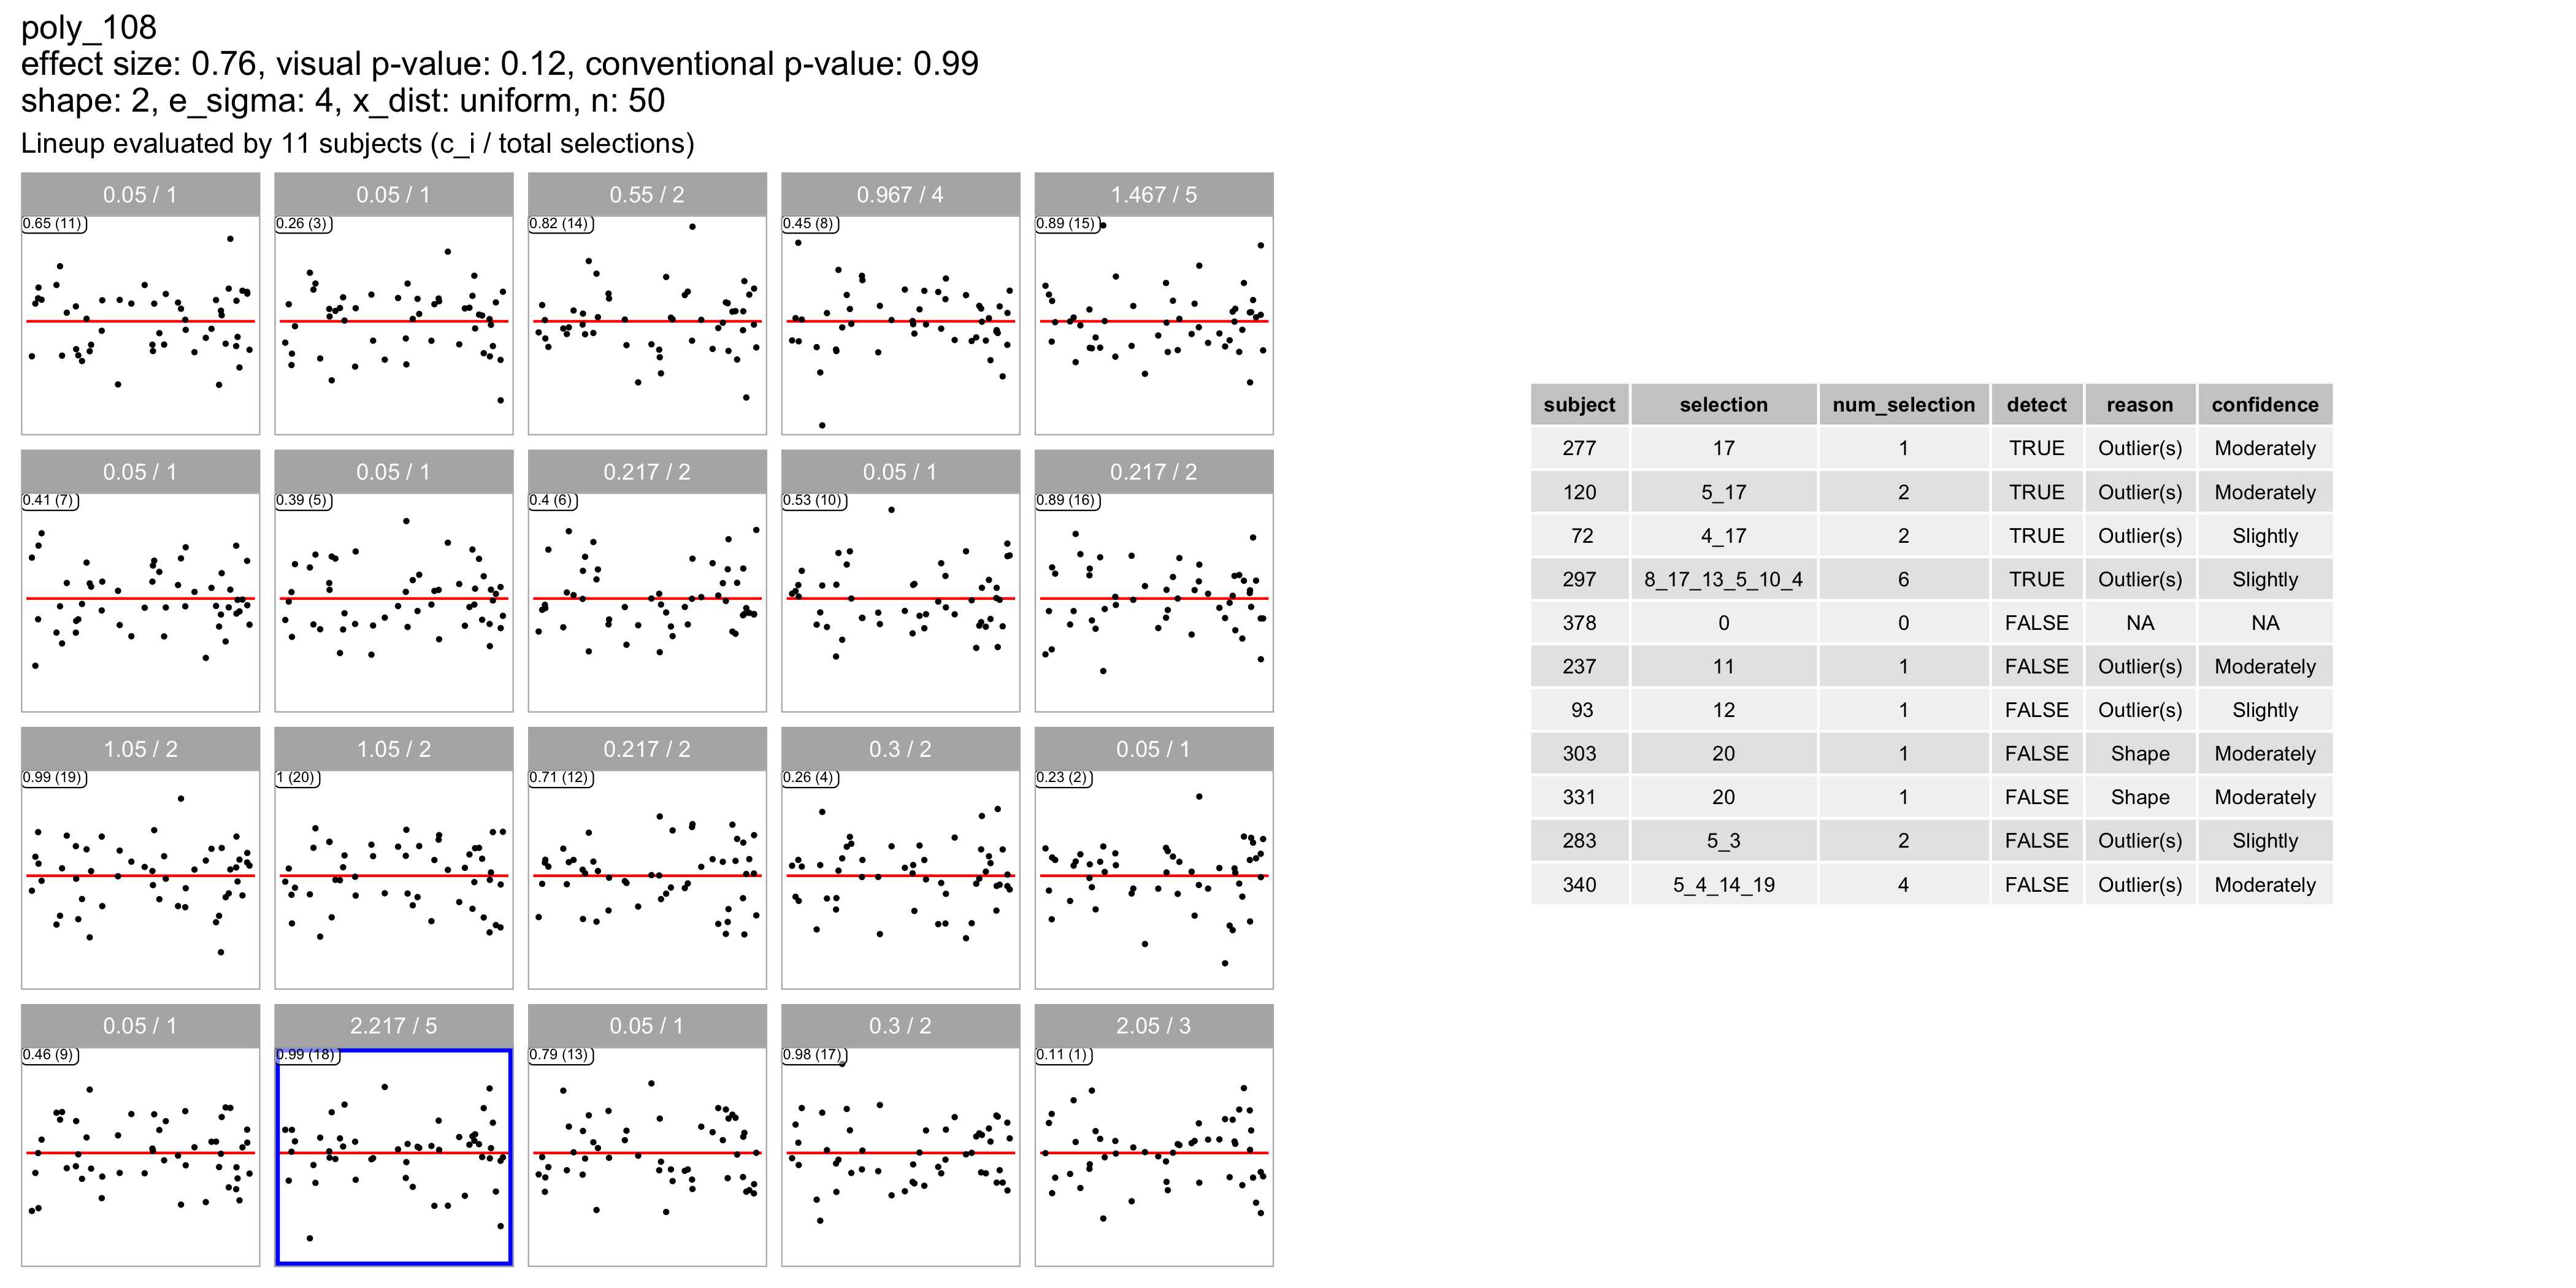
\includegraphics{thesis_files/figure-latex/unnamed-chunk-44-1.pdf}

\begin{verbatim}
## # A tibble: 2 x 2
##   type                 rate
##   <chr>               <dbl>
## 1 Cubic              0.0056
## 2 Heteroskedasticity 0.006
\end{verbatim}

\hypertarget{general-purpose-automatic-visual-statistical-inference-system}{%
\chapter{General Purpose Automatic Visual Statistical Inference System}\label{general-purpose-automatic-visual-statistical-inference-system}}

\hypertarget{visual-diagnostics-for-predictive-models-with}{%
\chapter{Visual Diagnostics for Predictive Models with \ldots{}}\label{visual-diagnostics-for-predictive-models-with}}

\hypertarget{timeline}{%
\chapter{Timeline}\label{timeline}}

\begin{table} \label{tab:timeline}
\centering
\begin{tabular}[t]{ll}
\toprule
\addlinespace[0.5em]
Date & Event\\
\addlinespace[0.5em]
\midrule
\addlinespace[0.5em]
\multicolumn{2}{l}{\textit{\textbf{2022}}}\\
\hspace{4em}March & Extend the scope of violations of classical normal linear\\ 
\addlinespace[0.5em]
\hspace{4em} & regression considered by the computer vision model\\
\addlinespace[0.5em]
\hspace{4em}April & Conduct human subject experiment on the extended model\\ 
\addlinespace[0.5em]
\hspace{4em} & defects\\
\addlinespace[0.5em]
\hspace{4em}May & Conclude the first project: draft and submit the first paper\\
\addlinespace[0.5em]
\hspace{4em}June & Review previous studies in image comparison\\
\addlinespace[0.5em]
\hspace{4em}July & Draft a new automatic visual inference system based\\
\addlinespace[0.5em]
\hspace{4em} & on image comparison\\
\addlinespace[0.5em]
\hspace{4em}August - November & Build the automatic system\\
\addlinespace[0.5em]
\hspace{4em}November - December & Conduct human subject experiment for validating the\\
\addlinespace[0.5em]
\hspace{4em} & automatic system\\
\addlinespace[0.5em]
\hspace{4em}December & Attend the Australasian Applied Statistics Conference\\
\addlinespace[0.5em]
\hline
\addlinespace[0.5em]
\multicolumn{2}{l}{\textit{\textbf{2023}}}\\
\hspace{4em}January - March & Finish the second project: prepare milestone material and\\
\addlinespace[0.5em]
\hspace{4em} & submit the second paper\\
\addlinespace[0.5em]
\hspace{4em}April - December & Apply the automatic visual inference system to predictive\\
\addlinespace[0.5em]
\hspace{4em} & model diagnostics\\
\addlinespace[0.5em]
\hline
\addlinespace[0.5em]
\multicolumn{2}{l}{\textit{\textbf{2024}}}\\
\hspace{4em}January - March & Finish the third project: finalize the thesis\\
\addlinespace[0.5em]
\bottomrule
\end{tabular}
\end{table}

\printbibliography[heading=bibintoc]



\end{document}
